\documentclass[man,floatsintext]{apa7}
% ---- Codificación y lenguaje ----
\usepackage[T1]{fontenc}
\usepackage[utf8]{inputenc}
\usepackage[spanish]{babel}
\decimalpoint

% ---- Citas y bibliografía (biblatex + APA) ----
\usepackage{csquotes}
\usepackage[style=apa,sortcites=true,sorting=nyt,backend=biber]{biblatex}
\DeclareLanguageMapping{spanish}{spanish-apa}

% ---- Matemáticas y utilidades ----
\usepackage{amsmath, amssymb}
\usepackage{xcolor}
\usepackage{colortbl}
\usepackage{geometry}
\geometry{letterpaper, margin=1in}
\usepackage{graphicx}
\usepackage{float}
\usepackage{caption}
\usepackage{booktabs}
\usepackage{tabularx}
\usepackage{microtype}
% ---- Hipervínculos ----
\usepackage{hyperref}
\hypersetup{
    colorlinks=true,
    breaklinks=true,
    linkcolor=blue,
    urlcolor=blue,
    citecolor=blue
}
\Urlmuskip=0mu plus 1mu\relax
\setlength{\emergencystretch}{6em}

%%%%%%%%%%%%%%%%%%%%%%%%%%%%%%%%%%%%%%%%%%%%%%%%%%%%%%%%%%%%%%%%%%%%%%%%%%%%%%%%%%%%%%%%%%%%%%%%%%%%%%%%%%%%%%%%%%%%%%%%%%%%%%%%%%%%%%%%%%%%%%%%%%%%%%%%%%%%%%%%%%%%%%%%%%%%%%%%%%%%%%%%%%%%%%
%%%%%%%%%%%%%%%%%%%%%%%%%%%%%%%%%%%%%%%%%%%%%%%%%%%%%%%%%%%%%%%%%%%%%%%%%%%%%%%%%%%%%%%%%%%%%%%%%%%%%%%%%%%%%%%%%%%%%%%%%%%%%%%%%%%%%%%%%%%%%%%%%%%%%%%%%%%%%%%%%%%%%%%%%%%%%%%%%%%%%%%%%%%%%%
\title{Universidad Panamericana\\ 
Maestría en Ciencia de Datos\\ 
Econometría\\ \vspace{0.5cm} 
Proyecto Final: Determinantes de Victorias en MLB
}
\shorttitle{Determinantes de Victorias en MLB}
\author{Enrique Ulises Báez Gómez Tagle,
    Luis Alejandro Guillén Alvarez\\
    Grupo 2
}
\affiliation{Universidad Panamericana}
\date{\today}
%%%%%%%%%%%%%%%%%%%%%%%%%%%%%%%%%%%%%%%%%%%%%%%%%%%%%%%%%%%%%%%%%%%%%%%%%%%%%%%%%%%%%%%%%%%%%%%%%%%%%%%%%%%%%%%%%%%%%%%%%%%%%%%%%%%%%%%%%%%%%%%%%%%%%%%%%%%%%%%%%%%%%%%%%%%%%%%%%%%%%%%%%%%%%%
%%%%%%%%%%%%%%%%%%%%%%%%%%%%%%%%%%%%%%%%%%%%%%%%%%%%%%%%%%%%%%%%%%%%%%%%%%%%%%%%%%%%%%%%%%%%%%%%%%%%%%%%%%%%%%%%%%%%%%%%%%%%%%%%%%%%%%%%%%%%%%%%%%%%%%%%%%%%%%%%%%%%%%%%%%%%%%%%%%%%%%%%%%%%%%
\begin{document}

\maketitle

\tableofcontents

\newpage
%%%%%%%%%%%%%%%%%%%%%%%%%%%%%%%%%%%%%%%%%%%%%%%%%%%%%%%%%%%%%%%%%%%%%%%%%%%%%%%%%%%%%%%%%%%%%%%%%%%%%%%%%%%%%%%%%%%%%%%%%%%%%%%%%%%%%%%%%%%%%%%%%%%%%%%%%%%%%%%%%%%%%%%%%%%%%%%%%%%%%%%%%%%%%%
%%%%%%%%%%%%%%%%%%%%%%%%%%%%%%%%%%%%%%%%%%%%%%%%%%%%%%%%%%%%%%%%%%%%%%%%%%%%%%%%%%%%%%%%%%%%%%%%%%%%%%%%%%%%%%%%%%%%%%%%%%%%%%%%%%%%%%%%%%%%%%%%%%%%%%%%%%%%%%%%%%%%%%%%%%%%%%%%%%%%%%%%%%%%%%
\section{Introducción}
% 
\subsection{Objetivo del trabajo:}
El propósito de este trabajo es aplicar un análisis de \textbf{regresión lineal múltiple} para explicar y pronosticar el número de \textbf{victorias (W)} de un equipo de Grandes Ligas en una temporada a partir de \emph{múltiples} variables explicativas consideradas de forma \emph{simultánea}. El modelo tendrá la forma general
\[
W_i=\beta_0+\beta_1 X_{1i}+\beta_2 X_{2i}+\beta_3 X_{3i}+\varepsilon_i,
\]
donde $X_{1},X_{2},X_{3}$ representan predictores de desempeño ofensivo y defensivo (\texttt{RunDiff}, \texttt{ERA}, \texttt{HR}). Los objetivos específicos son: (i) cuantificar los \emph{efectos marginales} de cada predictor sobre $W$; (ii) evaluar su significancia estadística y la bondad de ajuste del modelo; y (iii) generar pronósticos con intervalos de predicción para nuevas observaciones.
%
%%%%%%%%%%%%%%%%%%%%%%%%%%%%%%%%%%%%%%%%%%%%%%%%%%%%%%%%%%%%%%%%%%%%%%%%%%%%%%%%%%%%%%%%%%%%%%%%%%%%%%%%%%%%%%%%%%%%%%%%%%%%%%%%%%%%%%%%%%%%%%%%%%%%%%%%%%%%%%%%%%%%%%%%%%%%%%%%%%%%%%%%%%%%%%
%
\subsection{Justificación:}
Se adopta una especificación \textbf{múltiple} porque permite estimar el efecto \emph{parcial} de cada variable sobre $W$ controlando por las demás, reduciendo el sesgo por omisión inherente a modelos univariados. En particular:
\begin{itemize}
    \item \textbf{Diferencia de carreras (RunDiff = R - RA):} refleja la solidez ofensiva y defensiva combinada; se espera una relación positiva con las victorias.
    \item \textbf{ERA (Earned Run Average):} mide la calidad del pitcheo, donde un menor valor debería asociarse con más victorias (relación negativa).
    \item \textbf{Jonrones (HR):} indicador clave del poder ofensivo; se espera una relación positiva con las victorias.
\end{itemize}
Este enfoque permite comparar la \emph{relevancia relativa} de los predictores (magnitud y significancia), mejorar el desempeño predictivo frente a especificaciones simples y verificar rigurosamente los supuestos del modelo (linealidad conjunta, independencia, homocedasticidad, normalidad de residuos), además de diagnosticar \emph{multicolinealidad} mediante VIF.
%
%%%%%%%%%%%%%%%%%%%%%%%%%%%%%%%%%%%%%%%%%%%%%%%%%%%%%%%%%%%%%%%%%%%%%%%%%%%%%%%%%%%%%%%%%%%%%%%%%%%%%%%%%%%%%%%%%%%%%%%%%%%%%%%%%%%%%%%%%%%%%%%%%%%%%%%%%%%%%%%%%%%%%%%%%%%%%%%%%%%%%%%%%%%%%%
\subsection{Descripción de los datos:}
Se utiliza la Base de Datos de Béisbol de Lahman 1871-2024, publicada por la Society for American Baseball Research (SABR) con datos recopilados por Sean Lahman. La base está disponible en formato CSV, y específicamente se emplea el archivo \texttt{Teams.csv}, que contiene estadísticas anuales de desempeño de cada equipo de Grandes Ligas . 

El archivo original incluye 48 columnas y 3075 observaciones, correspondientes a temporadas desde 1871 hasta 2024. Sin embargo, para este trabajo se decidió filtrar únicamente los equipos de las ligas Americana (AL) y Nacional (NL), ya que representan las ligas principales de las Grandes Ligas de Béisbol y permiten obtener datos más homogéneos en términos de reglas y estructura competitiva. Asimismo, se seleccionó el periodo 2000-2019 porque corresponde a una etapa reciente del béisbol moderno, con un calendario estable de 162 juegos por temporada y sin las distorsiones que generó la temporada 2020 por la pandemia de COVID-19. Con este filtro se obtuvieron 600 observaciones (30 equipos por temporada durante 20 años), lo cual asegura un tamaño de muestra suficiente para aplicar análisis con validez estadística.

El dataset maestro conserva las siguientes variables principales:
\begin{itemize}
    \item Identificadores: \texttt{yearID}, \texttt{lgID}, \texttt{teamID}, \texttt{franchID}, \texttt{name}, \texttt{team\_year}, \texttt{season\_date}.
    \item Resultados: \texttt{W} (victorias), \texttt{L} (derrotas), \texttt{G} (juegos jugados).
    \item Estadísticas de desempeño: \texttt{R} (carreras anotadas), \texttt{RA} (carreras permitidas), \texttt{ERA} (efectividad), \texttt{HR} (jonrones).
    \item Variables derivadas: \texttt{RunDiff = R - RA}, \texttt{logHR1 = ln(HR+1)}.
\end{itemize}

El dataset es de tipo panel (equipo–año), con una observación por equipo por temporada; con esto es posible ajustar y evaluar un modelo de regresión múltiple, además de realizar análisis descriptivos y de correlación.
%%%%%%%%%%%%%%%%%%%%%%%%%%%%%%%%%%%%%%%%%%%%%%%%%%%%%%%%%%%%%%%%%%%%%%%%%%%%%%%%%%%%%%%%%%%%%%%%%%%%%%%%%%%%%%%%%%%%%%%%%%%%%%%%%%%%%%%%%%%%%%%%%%%%%%%%%%%%%%%%%%%%%%%%%%%%%%%%%%%%%%%%%%%%%%
%%%%%%%%%%%%%%%%%%%%%%%%%%%%%%%%%%%%%%%%%%%%%%%%%%%%%%%%%%%%%%%%%%%%%%%%%%%%%%%%%%%%%%%%%%%%%%%%%%%%%%%%%%%%%%%%%%%%%%%%%%%%%%%%%%%%%%%%%%%%%%%%%%%%%%%%%%%%%%%%%%%%%%%%%%%%%%%%%%%%%%%%%%%%%%
\section{Selección de Variables}
\subsection{Variable dependiente:}
La variable dependiente seleccionada es el número de \textbf{victorias (W)} que obtiene cada equipo de las Grandes Ligas de Béisbol (MLB) en una temporada regular. Esta variable representa de manera directa el desempeño global de un equipo, ya que ganar más partidos es el objetivo principal dentro de una temporada. A partir de ella se busca explicar qué factores de rendimiento ofensivo y defensivo tienen mayor influencia en el éxito deportivo.
%%%%%%%%%%%%%%%%%%%%%%%%%%%%%%%%%%%%%%%%%%%%%%%%%%%%%%%%%%%%%%%%%%%%%%%%%%%%%%%%%%%%%%%%%%%%%%%%%%%%%%%%%%%%%%%%%%%%%%%%%%%%%%%%%%%%%%%%%%%%%%%%%%%%%%%%%%%%%%%%%%%%%%%%%%%%%%%%%%%%%%%%%%%%%%
\subsection{Variables independientes:}
Para el análisis de regresión múltiple se consideran, de forma simultánea, tres variables explicativas:
%%%%%%%%%%%%%%%%%%%%%%%%%%%%%%%%%%%%%%%%%%%%%%%%%%%%%%%%%%%%%%%%%%%%%%%%%%%%%%%%%%%%%%%%%%%%%%%%%%%%%%%%%%%%%%%%%%%%%%%%%%%%%%%%%%%%%%%%%%%%%%%%%%%%%%%%%%%%%%%%%%%%%%%%%%%%%%%%%%%%%%%%%%%%%%

\begin{itemize}
    \item \textbf{Diferencia de carreras (RunDiff = R - RA):} mide la diferencia entre las carreras anotadas (\texttt{R}) y las carreras permitidas (\texttt{RA}). Es un indicador directo del dominio de un equipo sobre sus rivales; se espera que un mayor diferencial de carreras se traduzca en un mayor número de victorias (\(\beta > 0\)). 
    \item \textbf{ERA (Earned Run Average):} representa el promedio de carreras limpias permitidas por cada nueve entradas lanzadas. Es una métrica clave de la calidad del pitcheo: un valor más bajo de ERA refleja un mejor desempeño de los lanzadores y, por lo tanto, debería estar negativamente correlacionado con las derrotas y positivamente con las victorias (\(\beta < 0\)). 
    \item \textbf{Jonrones (HR):} corresponde al número total de cuadrangulares conectados por un equipo en una temporada. Dado que los jonrones aportan carreras directas, se espera que tengan una relación positiva con las victorias (\(\beta > 0\)).
\end{itemize}
%%%%%%%%%%%%%%%%%%%%%%%%%%%%%%%%%%%%%%%%%%%%%%%%%%%%%%%%%%%%%%%%%%%%%%%%%%%%%%%%%%%%%%%%%%%%%%%%%%%%%%%%%%%%%%%%%%%%%%%%%%%%%%%%%%%%%%%%%%%%%%%%%%%%%%%%%%%%%%%%%%%%%%%%%%%%%%%%%%%%%%%%%%%%%%
%%%%%%%%%%%%%%%%%%%%%%%%%%%%%%%%%%%%%%%%%%%%%%%%%%%%%%%%%%%%%%%%%%%%%%%%%%%%%%%%%%%%%%%%%%%%%%%%%%%%%%%%%%%%%%%%%%%%%%%%%%%%%%%%%%%%%%%%%%%%%%%%%%%%%%%%%%%%%%%%%%%%%%%%%%%%%%%%%%%%%%%%%%%%%%
\section{Análisis de Estadísticas Descriptivas}

\subsection{Medidas de tendencia central y dispersión:}
A partir del dateset maestro con las varibles y observaciones seleccionadas, se calculan las siguientes estadísticas descriptivas:
\begin{table}[H]
        \centering
        \caption{Estadísticas Descriptivas del dataset}
        \label{tab:desc_stats}
        \resizebox{\textwidth}{!}{
        \begin{tabular}{lrrrrrrrrrrr}
            \hline
                Variable & Count & Mean & Median & Mode & Std & Var & Min & Q1 & Q3 & IQR & Max \\
            \hline
                W       & 600 & 80.97 & 81.00 & 86.00 & 11.79 & 138.92 & 43.00 & 72.00 & 90.00 & 18.00 & 116.00 \\
                RunDiff & 600 & 0.00  & 2.00  & 54.00 & 111.11 & 12344.79 & -337.00 & -87.00 & 81.25 & 168.25 & 300.00 \\
                ERA     & 600 & 4.25  & 4.21  & 4.01  & 0.53  & 0.29 & 2.94 & 3.86 & 4.60 & 0.74 & 5.71 \\
                HR      & 600 & 173.47 & 170.00 & 161.00 & 36.87 & 1359.12 & 91.00 & 148.00 & 199.00 & 51.00 & 307.00 \\
                R       & 600 & 740.67 & 735.00 & 735.00 & 83.21 & 6924.21 & 513.00 & 684.00 & 795.25 & 111.25 & 978.00 \\
                RA      & 600 & 740.67 & 733.00 & 715.00 & 88.93 & 7909.25 & 525.00 & 676.75 & 804.00 & 127.25 & 981.00 \\
                G       & 600 & 161.96 & 162.00 & 162.00 & 0.31 & 0.10 & 161.00 & 162.00 & 162.00 & 0.00 & 163.00 \\
                L       & 600 & 80.97 & 80.50 & 76.00 & 11.76 & 138.34 & 46.00 & 72.00 & 90.00 & 18.00 & 119.00 \\
            \hline
        \end{tabular}
        }
    \end{table}

A continuación se detallan las características principales:

\begin{itemize}
    \item \textbf{Victorias (W):} En promedio los equipos ganan 81 juegos por temporada , con una desviación estándar de 11.8. El rango va de 43 a 116 victorias, lo que refleja tanto equipos altamente competitivos como equipos en el extremo opuesto.
    \item \textbf{Diferencia de carreras (RunDiff):} Tiene media cercana a cero, que sería esperado en un balance global de liga, pero una alta dispersión ($\approx 111$, rango de -337 a +300). Esto muestra que algunos equipos dominan ampliamente a sus rivales mientras otros son ampliamente superados.
    \item \textbf{ERA (Efectividad del pitcheo):} Promedia 4.25, con valores típicos entre 3.9 y 4.6 (IQR = 0.74). La dispersión es moderada y refleja diferencias en la calidad del pitcheo entre equipos, con casos extremos desde 2.94 hasta 5.71.
    \item \textbf{Jonrones (HR):} Los equipos conectan en promedio 173 cuadrangulares por temporada, con un rango entre 91 y 307. Esta variabilidad se ve reflejada por las distintas filosofías ofensivas.
    \item \textbf{Carreras anotadas (R) y recibidas (RA):} Ambas variables tienen media $\approx 741$, lo que es natural dado el equilibrio de la liga. Su dispersión ($\approx 83-89$) muestra diferencias en ofensiva y defensiva entre equipos.
    \item \textbf{Juegos (G):} Es prácticamente constante en 162, como dicta el calendario, con variaciones mínimas por suspensiones o ajustes.
    \item \textbf{Derrotas (L):} Presentan la misma estructura que las victorias, con media 81 y desviación de 11.7, dada la relación \(W+L \approx 162\).
\end{itemize}
%%%%%%%%%%%%%%%%%%%%%%%%%%%%%%%%%%%%%%%%%%%%%%%%%%%%%%%%%%%%%%%%%%%%%%%%%%%%%%%%%%%%%%%%%%%%%%%%%%%%%%%%%%%%%%%%%%%%%%%%%%%%%%%%%%%%%%%%%%%%%%%%%%%%%%%%%%%%%%%%%%%%%%%%%%%%%%%%%%%%%%%%%%%%%%
\subsection{Visualización de los datos:}

Con el fin de comprender mejor el comportamiento de las variables y su relación con las victorias, se generaron distintas visualizaciones: histogramas, boxplots, diagramas de dispersión, gráficas de pastel y una serie de tiempo de ejemplo.

\begin{figure}[H]
    \centering
    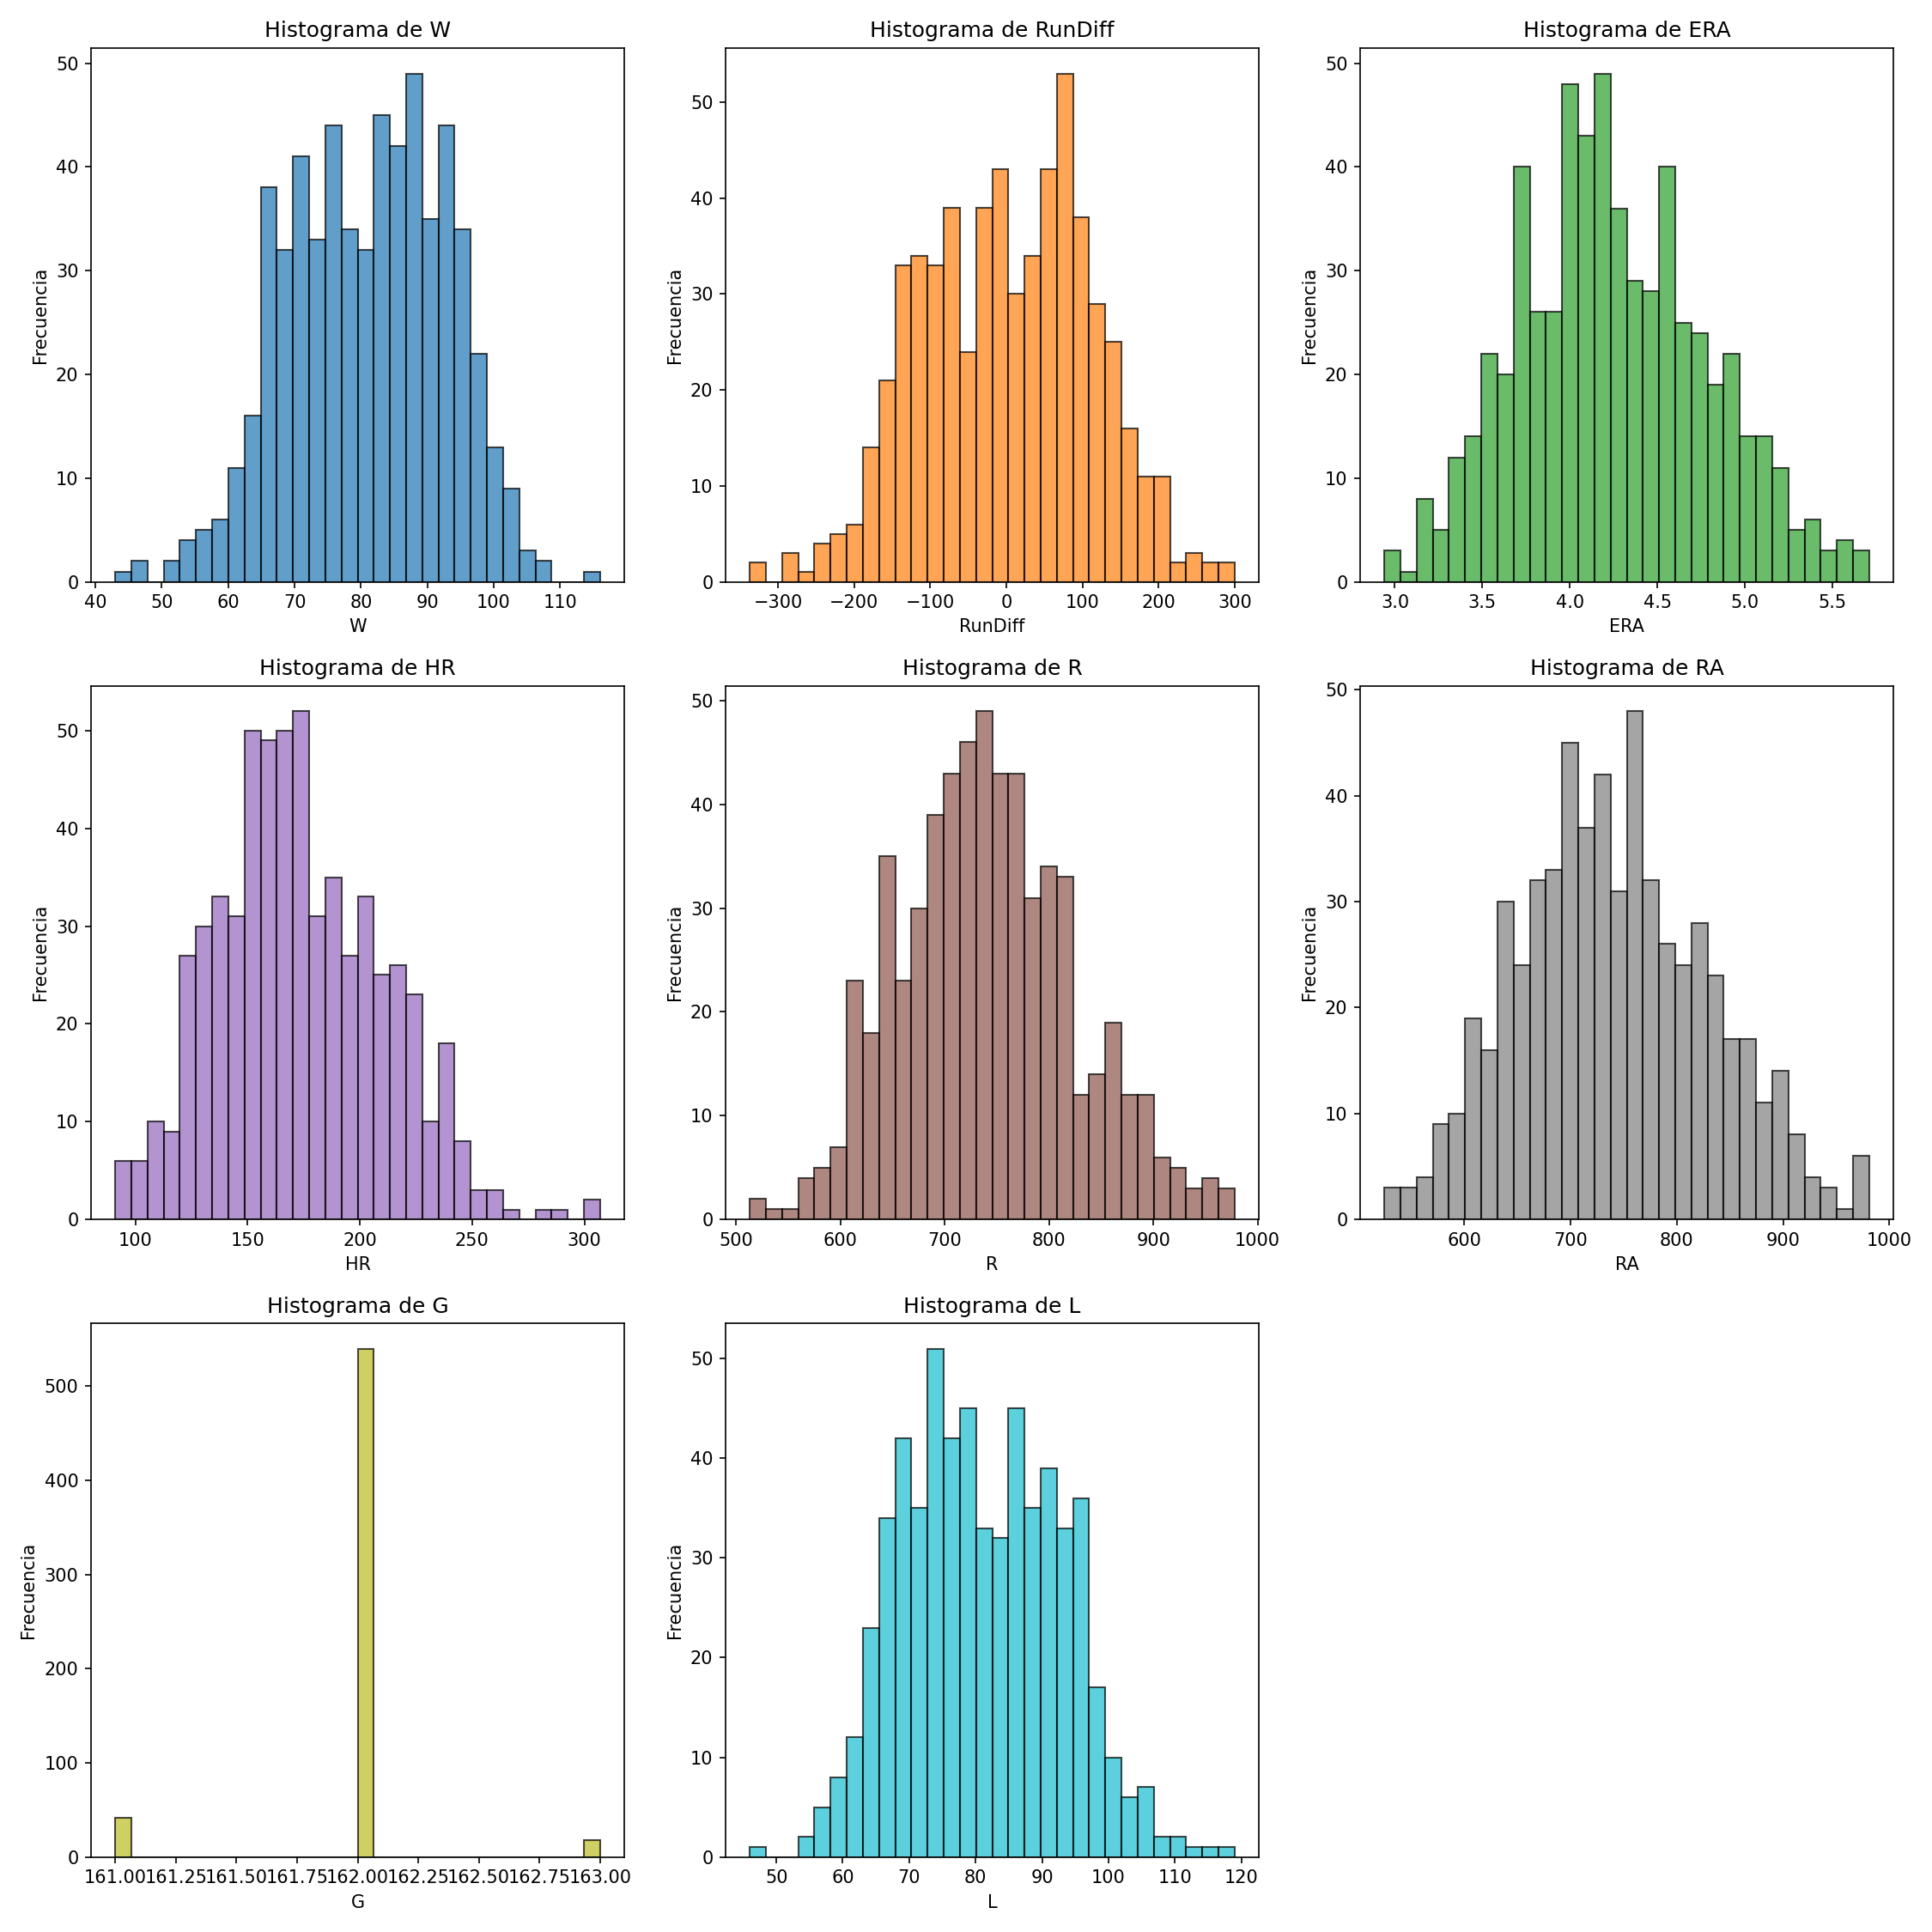
\includegraphics[width=0.65\textwidth]{../plots/final_version/all_histograms.png}
    \caption{Histogramas de W, RunDiff, ERA, HR, R, RA, G y L (2000--2019).}
\end{figure}

Los histogramas confirman distribuciones aproximadamente simétricas en \textbf{W} y \textbf{L}, con centro en 81 victorias/derrotas. 
\textbf{RunDiff} muestra gran dispersión, confirmarndo que algunos equipos superan a sus rivales por cientos de carreras, mientras otros son ampliamente superados. 
\textbf{ERA} se concentra en torno a 4, reflejando diferencias moderadas en pitcheo. 
\textbf{HR} se distribuye entre 100-300.
\textbf{R} y \textbf{RA} tienen formas parecidas, centradas cerca de 740, lo que refleja equilibrio ofensivo-defensivo en la liga. 
\textbf{G} es casi una constante en 162, validando la homogeneidad del calendario.

\begin{figure}[H]
    \centering
    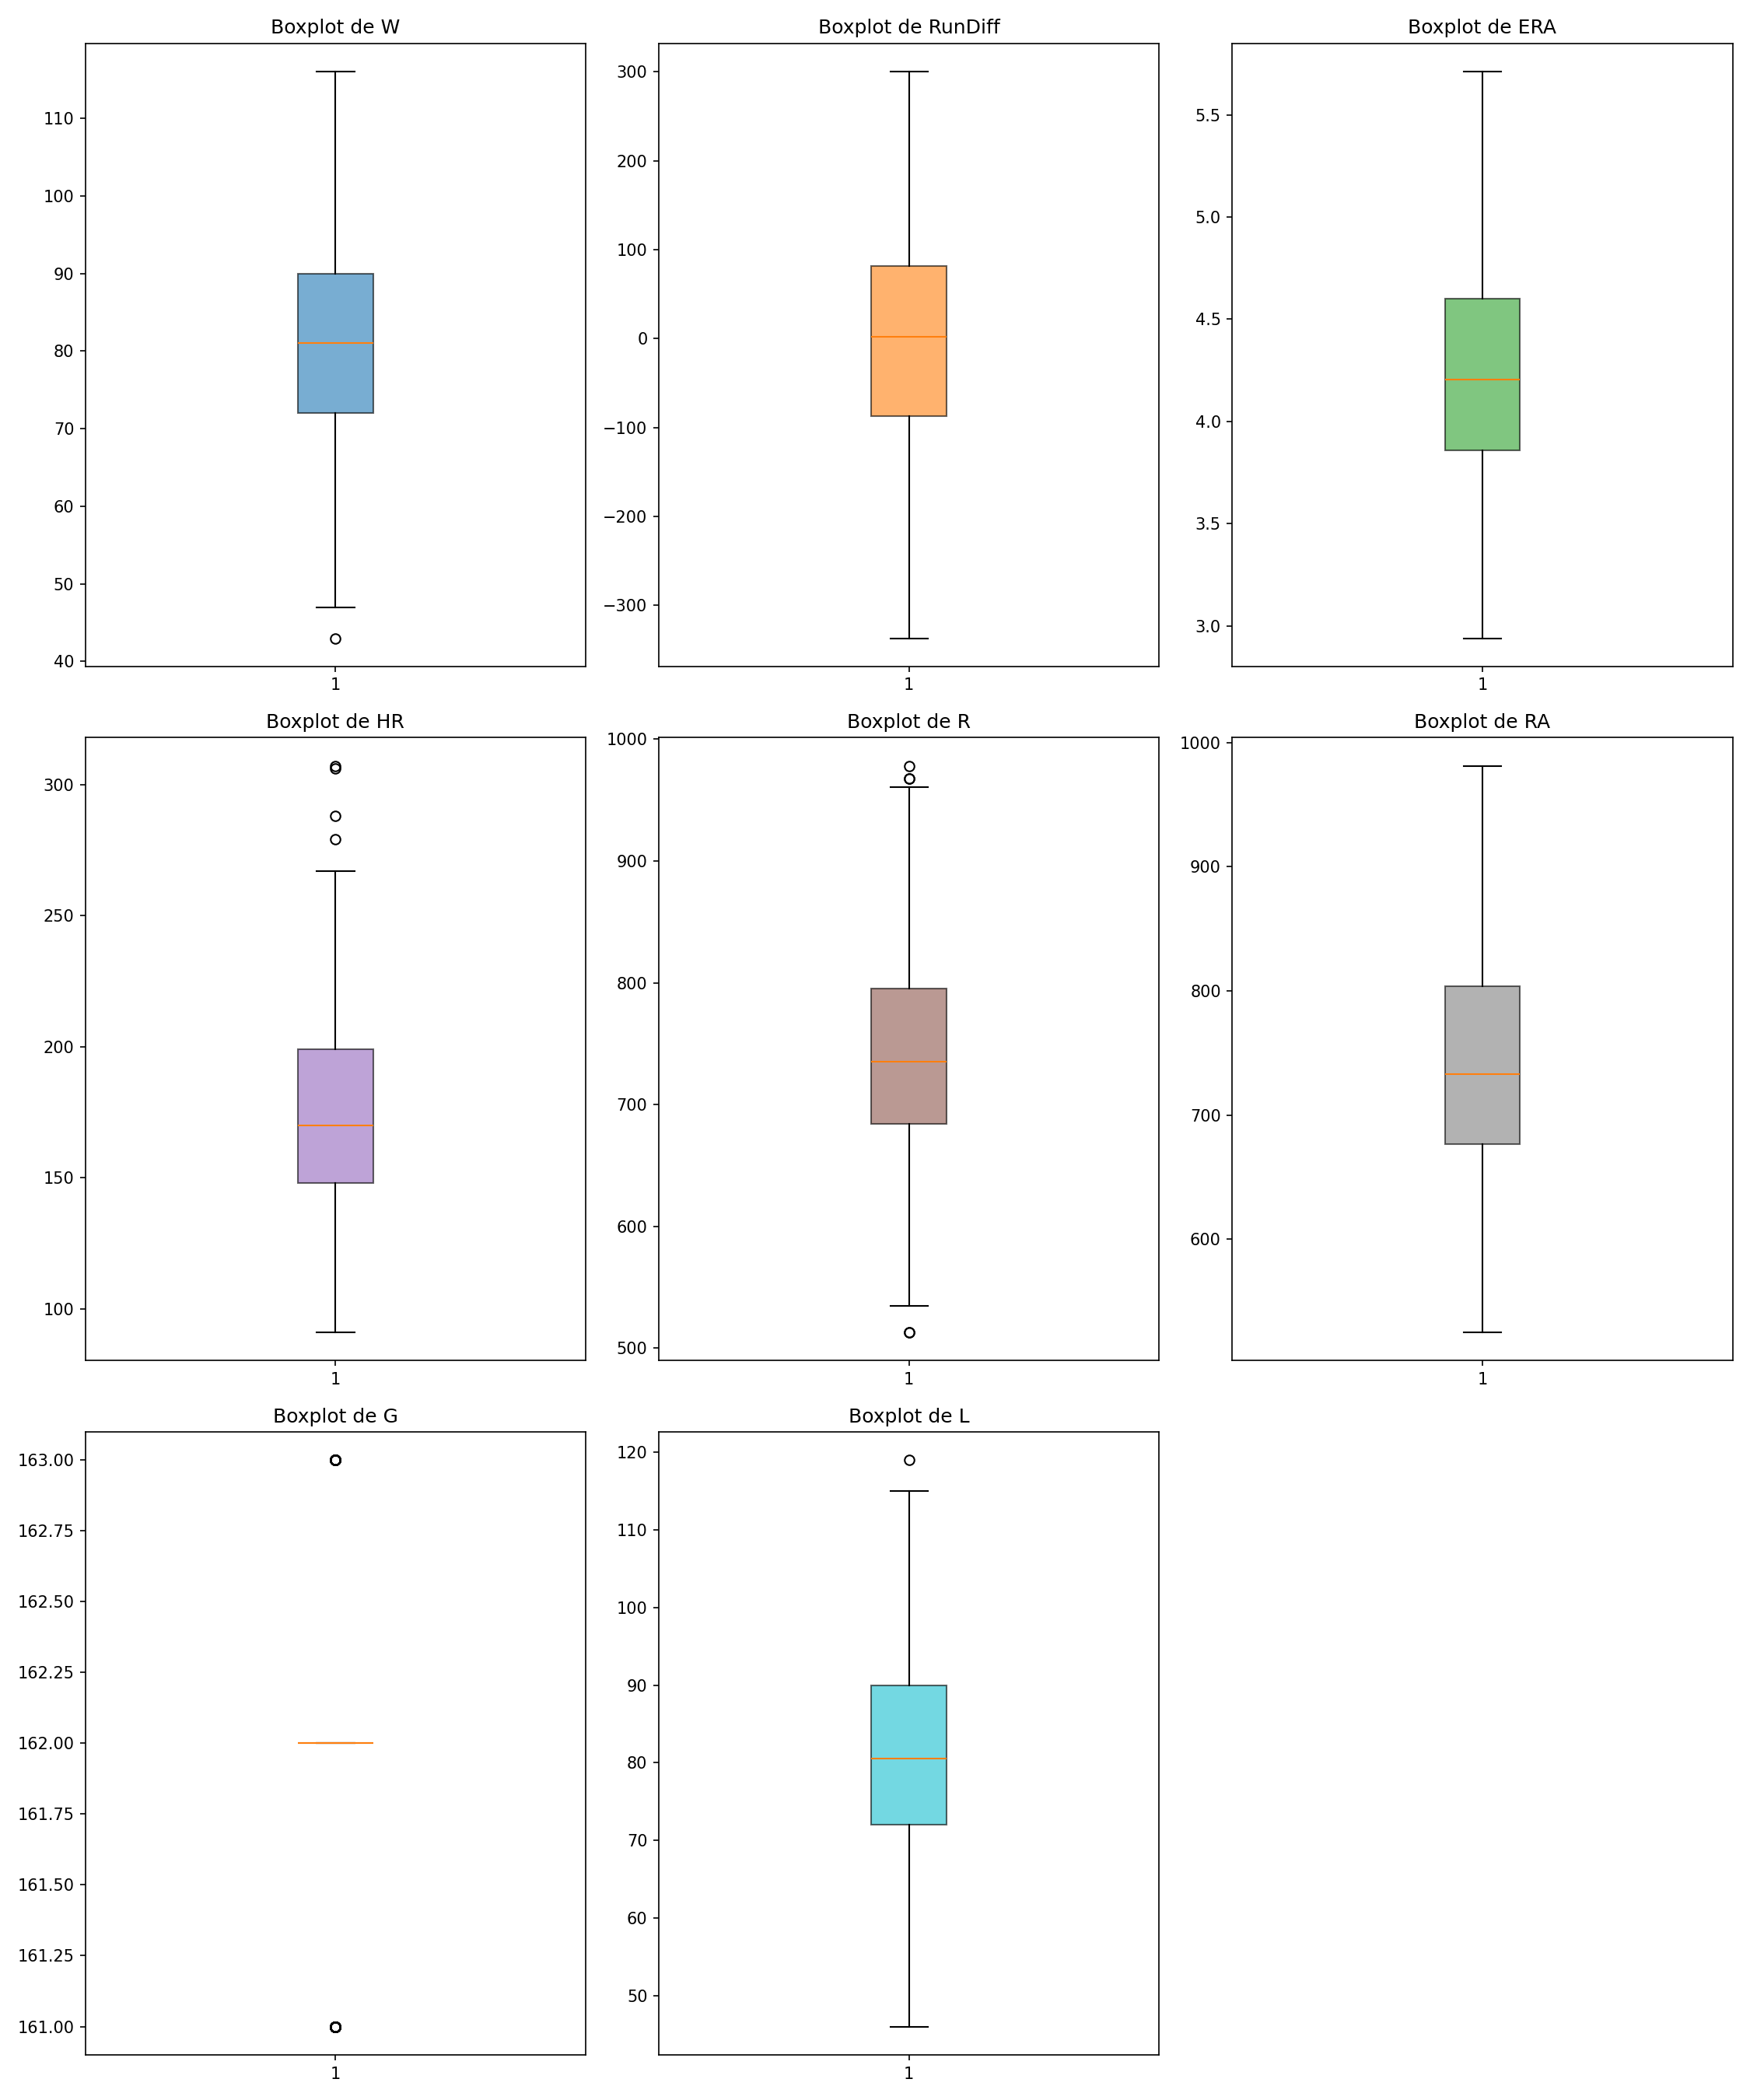
\includegraphics[width=0.7\textwidth]{../plots/final_version/all_boxplots.png}
    \caption{Boxplots por variable: dispersión, mediana y valores atípicos.}
\end{figure}

Los boxplots identifican \textit{outliers} relevantes: 
(i) en \textbf{HR}, equipos con poder ofensivo distintivo (300+ HR), 
(ii) en \textbf{R} se ven reflejados esos mismos casos extremos de producción ofensiva.
(iii) en \textbf{G}, ligeras desviaciones (161 o 163 partidos), explicadas por suspensiones o dobles juegos. 
En \textbf{RunDiff} se observan extremos tanto positivos como negativos, reflejando temporadas históricas dominantes o muy pobres.

\begin{figure}[H]
    \centering
    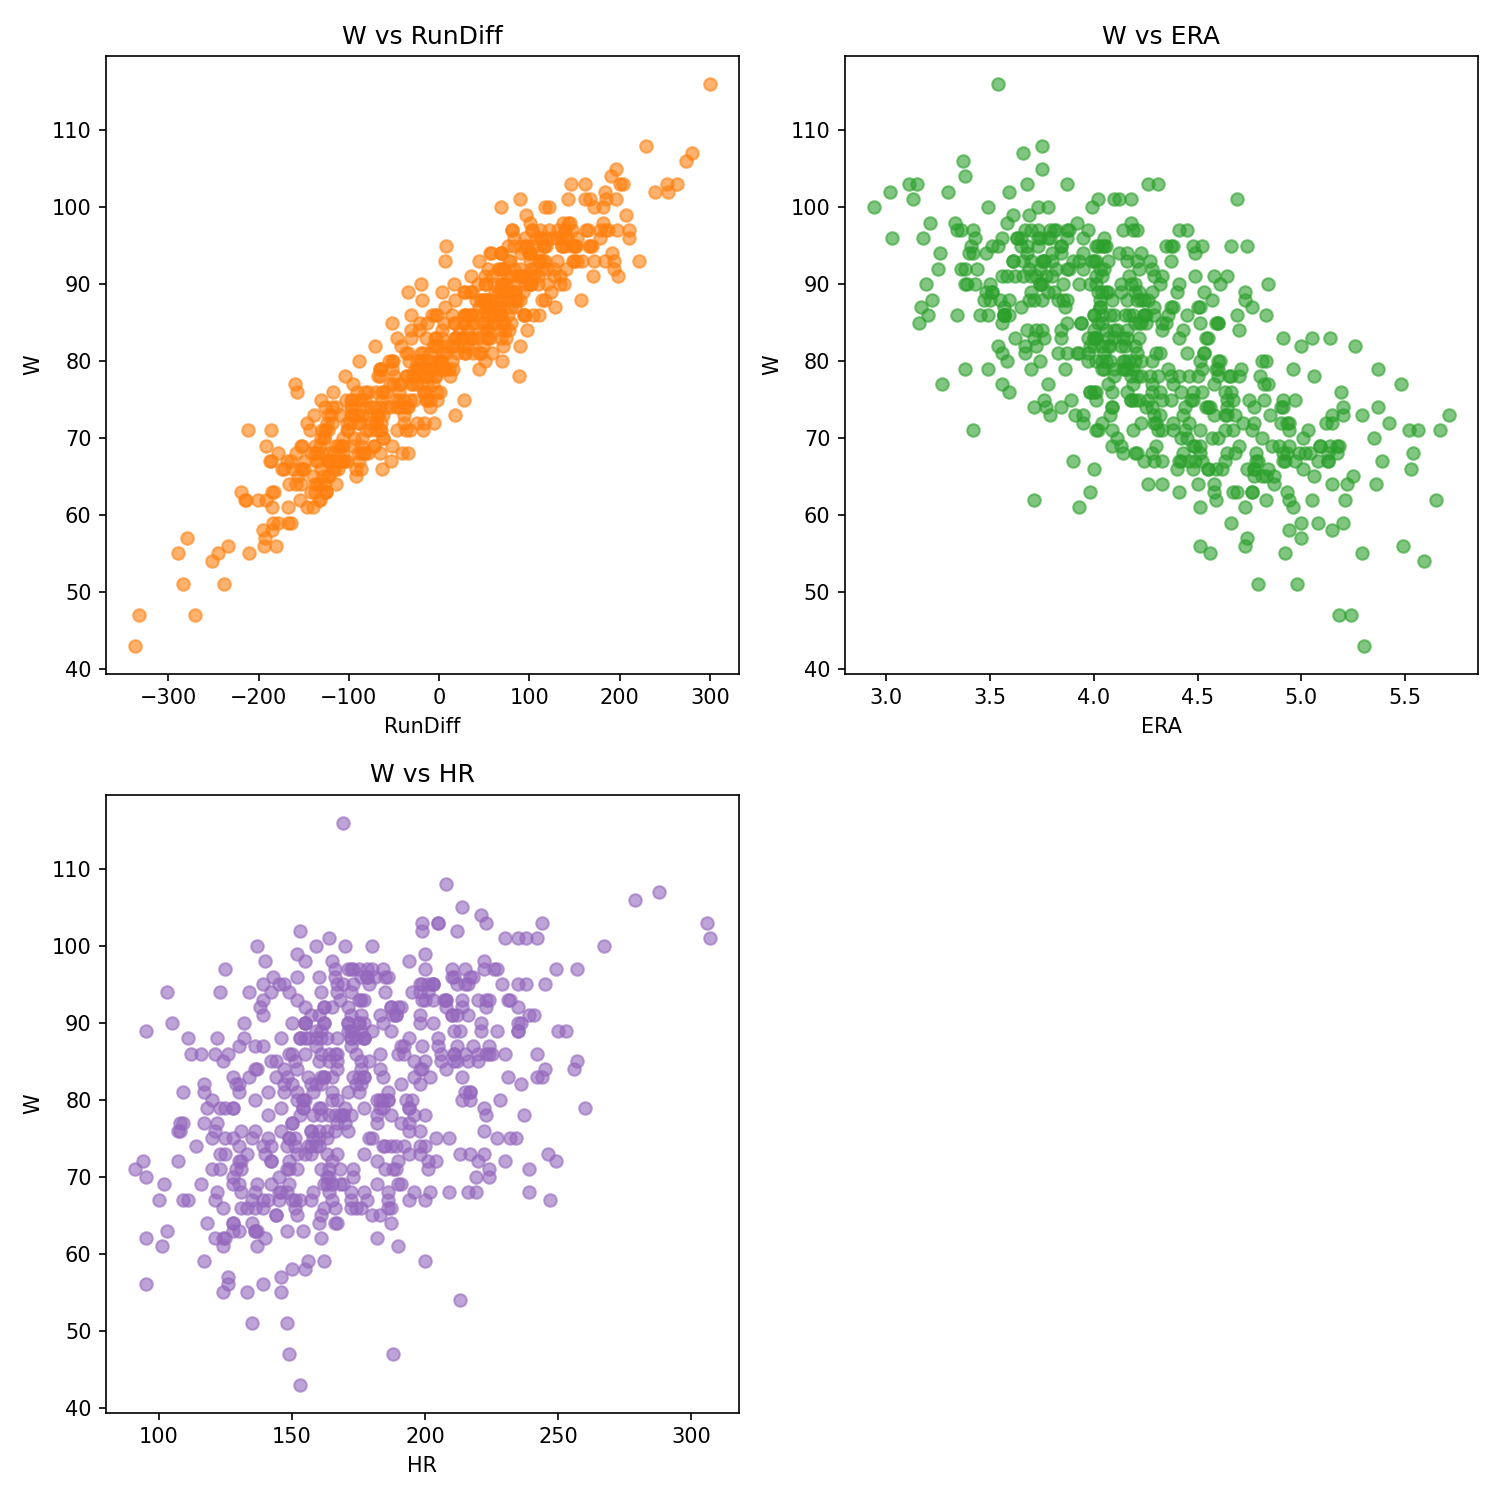
\includegraphics[width=\textwidth]{../plots/final_version/all_scatter_W.png}
    \caption{Diagramas de dispersión: W vs RunDiff, ERA y HR.}
\end{figure}

\textbf{W vs RunDiff} presenta la relación más fuerte y lineal: a mayor diferencial de carreras, más victorias, confirmando su validez como predictor central.  
\textbf{W vs ERA} muestra una relación negativa clara: equipos con menor efectividad del pitcheo (ERA baja) ganan más.  
\textbf{W vs HR} tiene asociación positiva pero más difusa; los cuadrangulares ayudan a ganar, aunque con variabilidad.


\begin{figure}[H]
    \centering
    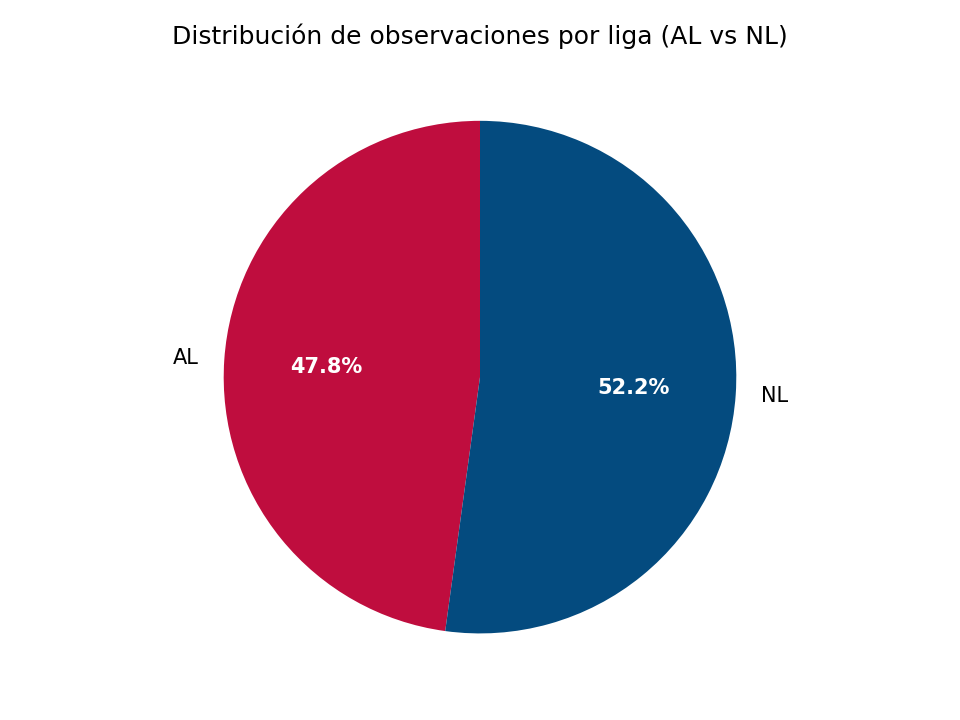
\includegraphics[width=0.6\textwidth]{../plots/final_version/pie_ligas_colored.png}
    \caption{Distribución de observaciones por liga (AL vs NL), 2000--2019.}
\end{figure}

El dataset está balanceado entre \textbf{NL} (52.2\%) y \textbf{AL} (47.8\%),y con esto se garantiza representatividad de ambas ligas, sin sesgos por desbalance en la muestra.

\begin{figure}[H]
    \centering
    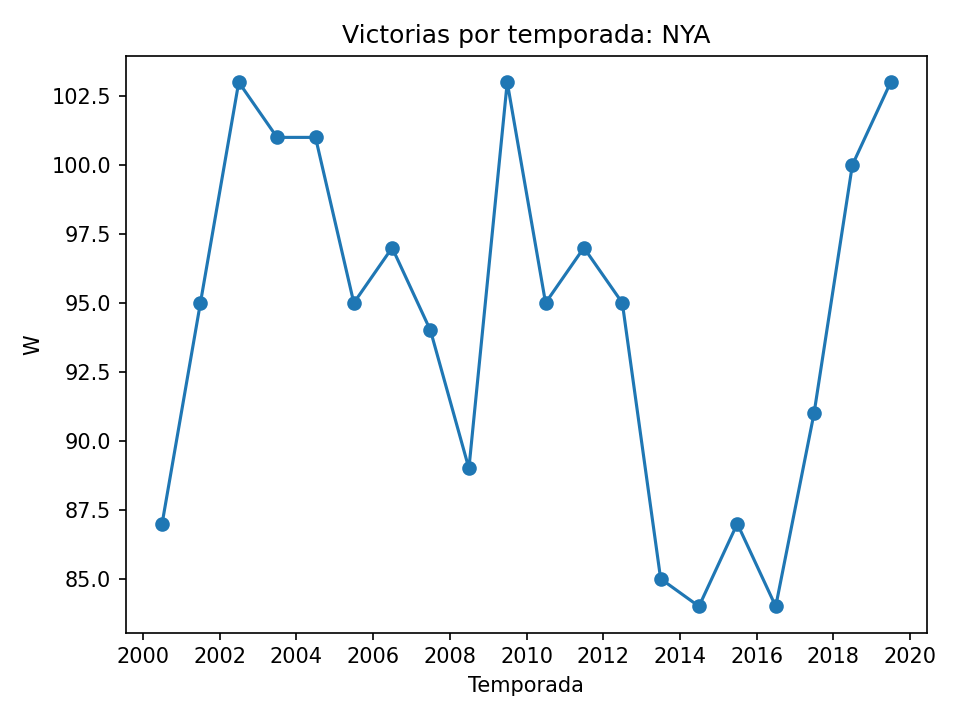
\includegraphics[width=0.8\textwidth]{../plots/ts_W_NYA.png}
    \caption{Serie de tiempo de victorias (ejemplo: NYA), 2000--2019.}
\end{figure}

Los Yankees de Nueva York (NYA) ilustran la variabilidad interanual en victorias. 
Se observan picos de más de 100 triunfos en varias temporadas y caídas a la franja de 85-90 victorias en otras. 
Este patrón muestra que incluso equipos consistentemente competitivos presentan fluctuaciones naturales, útiles para entender la estabilidad del modelo a lo largo del tiempo.

%%%%%%%%%%%%%%%%%%%%%%%%%%%%%%%%%%%%%%%%%%%%%%%%%%%%%%%%%%%%%%%%%%%%%%%%%%%%%%%%%%%%%%%%%%%%%%%%%%%%%%%%%%%%%%%%%%%%%%%%%%%%%%%%%%%%%%%%%%%%%%%%%%%%%%%%%%%%%%%%%%%%%%%%%%%%%%%%%%%%%%%%%%%%%%
\subsection{Identificación de valores atípicos:}

El análisis mediante el método del rango intercuartílico (IQR) permitió identificar observaciones atípicas en varias variables:

\begin{itemize}
    \item \textbf{Victorias (W):} El caso más extremo corresponde a los Detroit Tigers en 2003, con solo 43 victorias, claramente fuera del rango intercuartílico (45--117). Esto refleja una de las peores campañas en la historia reciente de MLB.
    \item \textbf{Jonrones (HR):} En 2019 se detectaron valores extraordinariamente altos en equipos como Minnesota Twins (307), New York Yankees (306), Houston Astros (288) y Los Angeles Dodgers (279), todos por encima del umbral superior (275.5). Esto coincide con el ``Año del jonrón''. en 2019, cuando se registró un récord colectivo histórico de cuadrangulares.
    \item \textbf{Carreras anotadas (R):} Se identifican equipos con valores extremos, por ejemplo, los Yankees (2007) y Rockies (2000) con más de 968 carreras, y los Marlins (2013) o Mariners (2010) con apenas 513, fuera del rango esperado (517--962).
    \item \textbf{Juegos disputados (G):} Aunque la liga establece un calendario de 162 juegos, se detectan temporadas con 161 o 163 partidos, resultado de suspensiones o reprogramaciones (e.g., Cubs 2009, Rockies 2007, Rangers 2013).
    \item \textbf{Derrotas (L):} Nuevamente destacan los Tigers de 2003, con 119 derrotas, simétrico al outlier en victorias.
\end{itemize}

Estos valores atípicos no necesariamente representan errores de medición, sino hechos históricos del béisbol (equipos en un muy bajo nivel, ofensivas históricas, o particularidades del calendario). Sin embargo, es importante tenerlos en cuenta porque pueden influir en el ajuste de los modelos de regresión, afectando los coeficientes e incrementando la dispersión residual.
%%%%%%%%%%%%%%%%%%%%%%%%%%%%%%%%%%%%%%%%%%%%%%%%%%%%%%%%%%%%%%%%%%%%%%%%%%%%%%%%%%%%%%%%%%%%%%%%%%%%%%%%%%%%%%%%%%%%%%%%%%%%%%%%%%%%%%%%%%%%%%%%%%%%%%%%%%%%%%%%%%%%%%%%%%%%%%%%%%%%%%%%%%%%%%
%%%%%%%%%%%%%%%%%%%%%%%%%%%%%%%%%%%%%%%%%%%%%%%%%%%%%%%%%%%%%%%%%%%%%%%%%%%%%%%%%%%%%%%%%%%%%%%%%%%%%%%%%%%%%%%%%%%%%%%%%%%%%%%%%%%%%%%%%%%%%%%%%%%%%%%%%%%%%%%%%%%%%%%%%%%%%%%%%%%%%%%%%%%%%%
\section{Análisis de Correlación}
\subsection{Correlación entre las variables:}

Se calculó el coeficiente de correlación de Pearson y Spearman entre el número de victorias (W) y las variables explicativas 
(RunDiff, ERA y HR). Los resultados se resumen en la Tabla \ref{tab:corr_w_x} y en las Figuras 
\ref{fig:heatmap_pearson}--\ref{fig:heatmap_spearman}.

\begin{center}
    \begin{table}
        \caption{Correlación de W con variables explicativas}
        \label{tab:corr_w_x}
        \begin{tabular}{lrrrrr}
            \toprule
            Variable & Pearson r & p (Pearson) & Spearman $\rho$ & p (Spearman) & N \\
            \midrule
            RunDiff & 0.9395 & 0.0000 & 0.9398 & 0.0000 & 600 \\
            HR & 0.3920 & 0.0000 & 0.3853 & 0.0000 & 600 \\
            ERA & -0.6554 & 0.0000 & -0.6575 & 0.0000 & 600 \\
            \bottomrule
        \end{tabular}
    \end{table}
\end{center}


\begin{figure}[H]
    \centering
    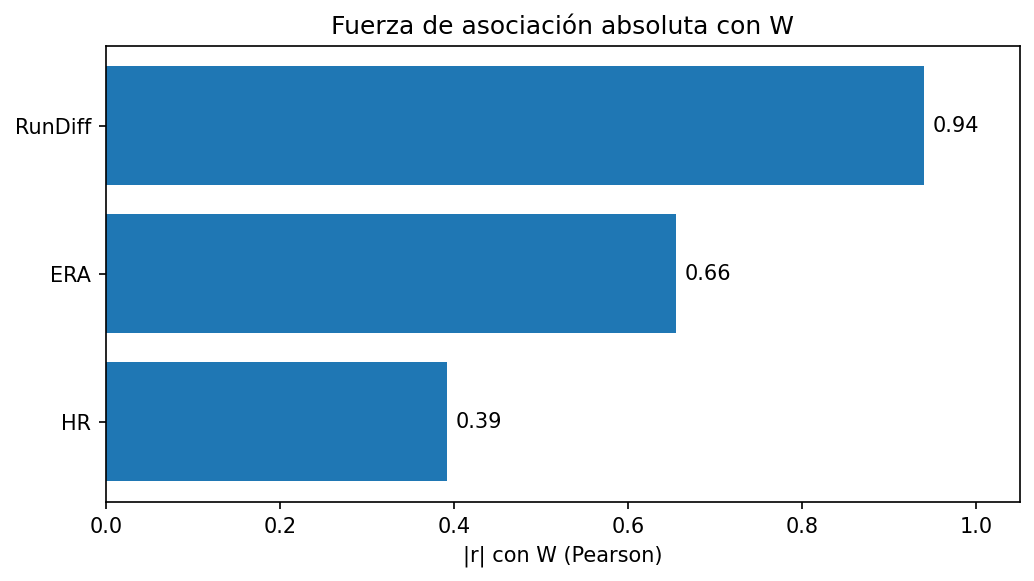
\includegraphics[width=0.75\textwidth]{../plots/final_version/bar_abs_r_W.png}
    \caption{Fuerza de asociación absoluta (|r|) de cada predictor con W (Pearson).}
    \label{fig:bar_abs_r}
\end{figure}

\subsection{Interpretación de los resultados}

\begin{itemize}
    \item \textbf{RunDiff} presenta la correlación más fuerte con $W (r = 0.94, p < 0.001)$, lo que confirma que la diferencia de carreras es un predictor casi determinístico del número de victorias.
    \item \textbf{ERA} muestra una correlación negativa alta $(r = -0.66, p < 0.001)$. Esto indica que un menor promedio de carreras limpias permitidas (mejor pitcheo) está fuertemente asociado con más victorias.
    \item \textbf{HR} exhibe una correlación positiva moderada $(r \approx 0.39, p < 0.001)$. Los jonrones ayudan a ganar, aunque no explican tanto como RunDiff o ERA.
\end{itemize}

\begin{figure}[H]
    \centering
    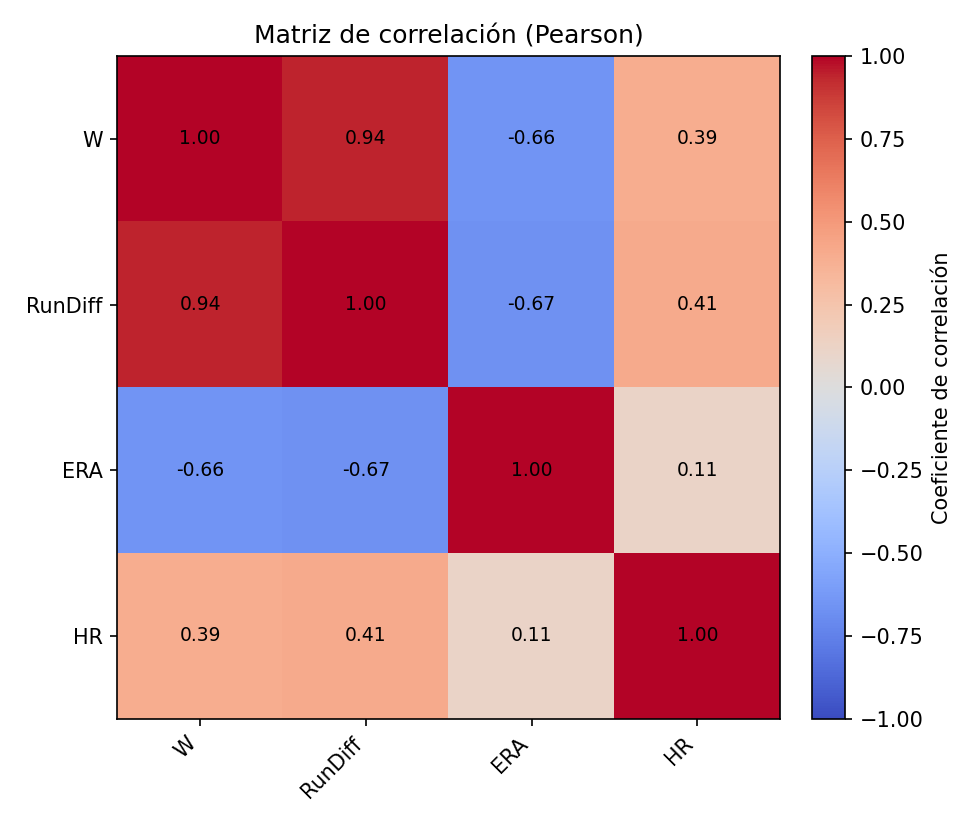
\includegraphics[width=0.6\textwidth]{../plots/final_version/heatmap_corr_pearson.png}
    \caption{Matriz de correlación (Pearson) entre W y las variables explicativas.}
    \label{fig:heatmap_pearson}
\end{figure}

\begin{figure}[H]
    \centering
    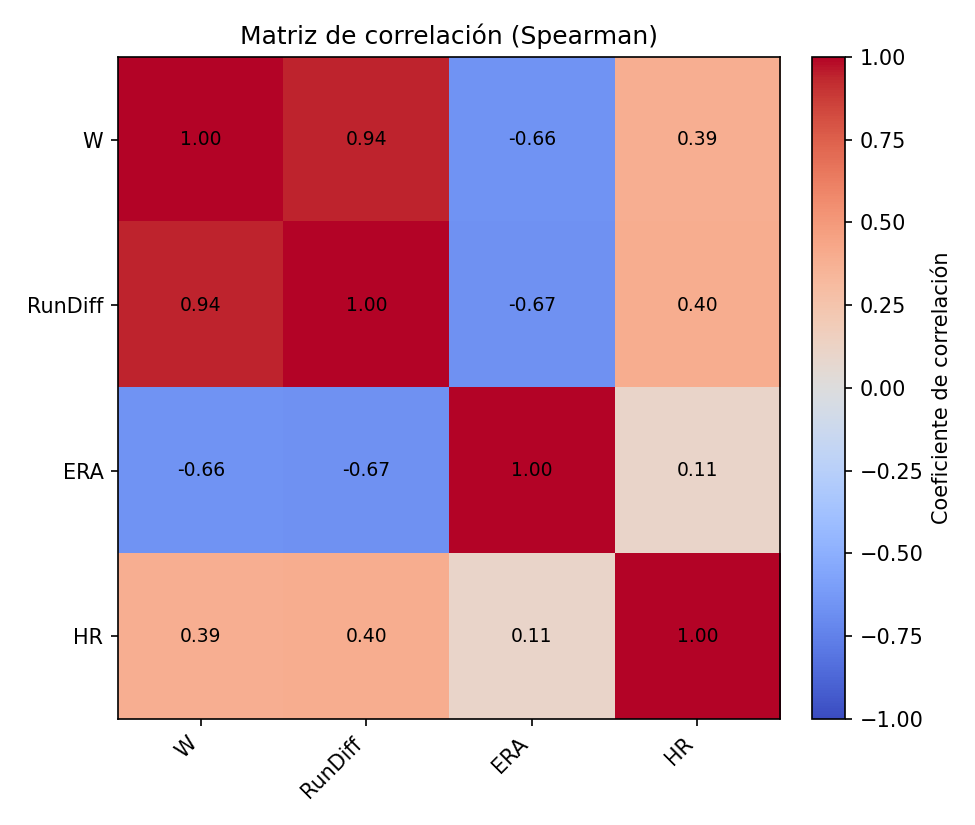
\includegraphics[width=0.6\textwidth]{../plots/final_version/heatmap_corr_spearman.png}
    \caption{Matriz de correlación (Spearman) entre W y las variables explicativas.}
    \label{fig:heatmap_spearman}
\end{figure}

Tanto Pearson como Spearman producen resultados consistentes: RunDiff y ERA son los predictores más fuertemente asociados con las victorias, mientras que los jonrones tienen un efecto más limitado. Esto anticipa que los modelos de regresión simple con RunDiff y ERA tendrán mayor poder explicativo que aquellos con HR.
%%%%%%%%%%%%%%%%%%%%%%%%%%%%%%%%%%%%%%%%%%%%%%%%%%%%%%%%%%%%%%%%%%%%%%%%%%%%%%%%%%%%%%%%%%%%%%%%%%%%%%%%%%%%%%%%%%%%%%%%%%%%%%%%%%%%%%%%%%%%%%%%%%%%%%%%%%%%%%%%%%%%%%%%%%%%%%%%%%%%%%%%%%%%%%
\section{Modelo de Regresión Múltiple}
\subsection{Especificación y ajuste}
El modelo estimado es:
\[
W_i = \beta_0 + \beta_1\,\text{RunDiff}_i + \beta_2\,\text{ERA}_i + \beta_3\,\text{HR}_i + \varepsilon_i,
\]
que se ajustó por Mínimos Cuadrados Ordinarios . Las siguientes figuras muestran, a modo exploratorio, las relaciones con $W$ y los residuales del ajuste (para evaluar linealidad y patrones):

\begin{figure}[H]
    \centering
    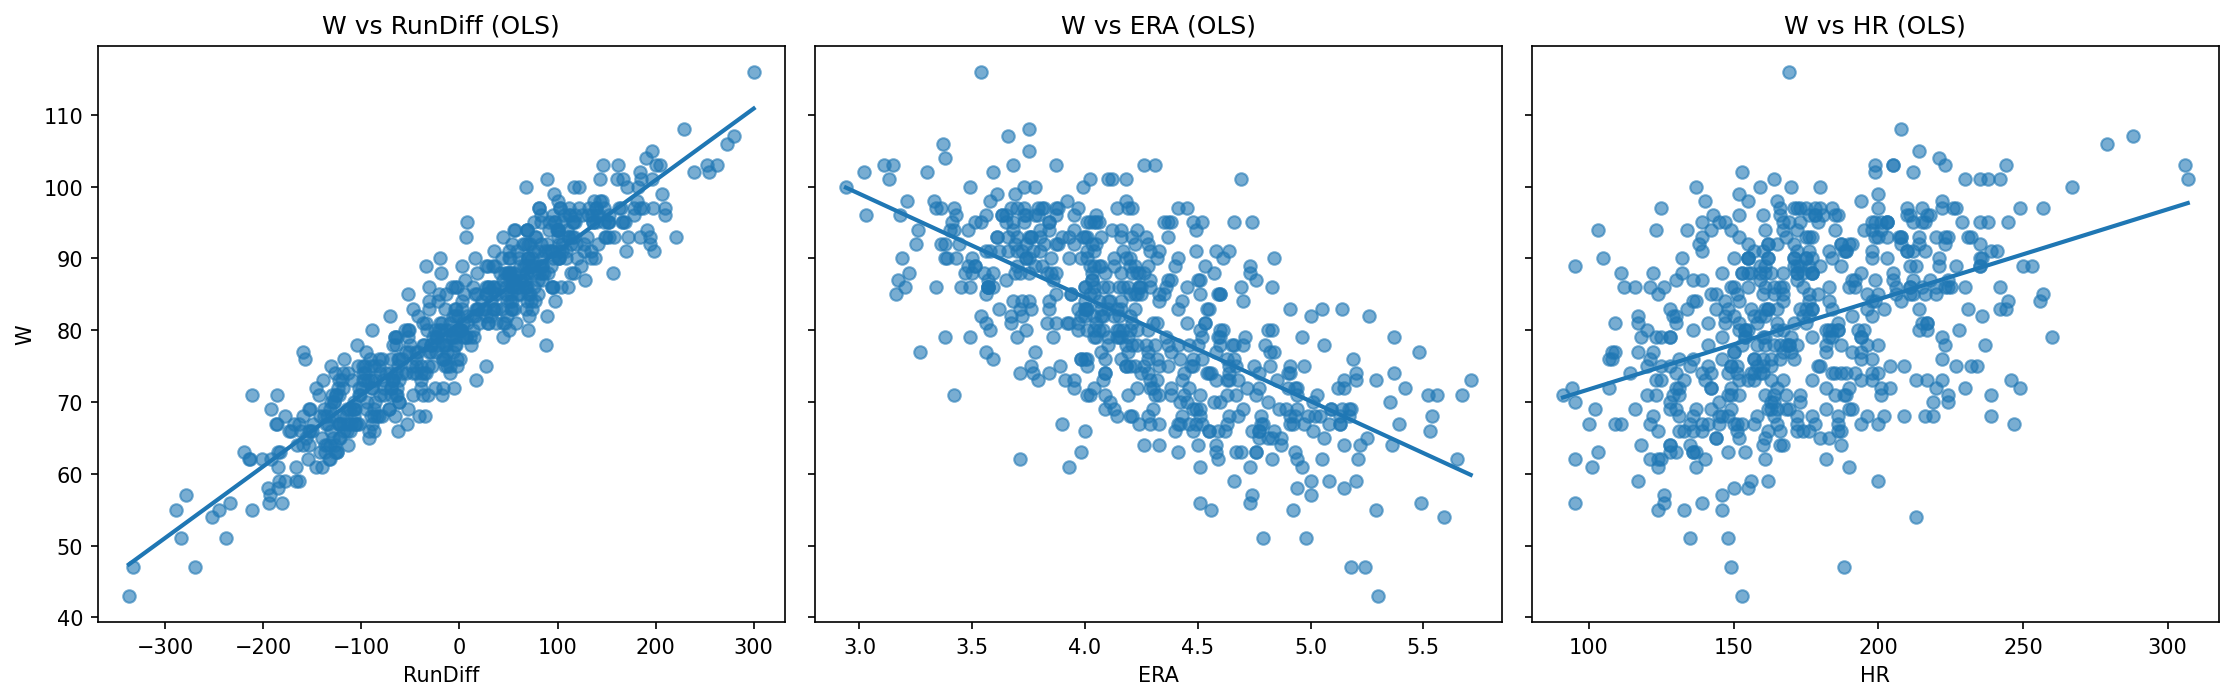
\includegraphics[width=\textwidth]{../plots/ols_scatter_grid_RunDiff_ERA_HR.png}
    \caption{Diagramas de dispersión: W vs RunDiff, ERA y HR .}
\end{figure}

\begin{figure}[H]
    \centering
    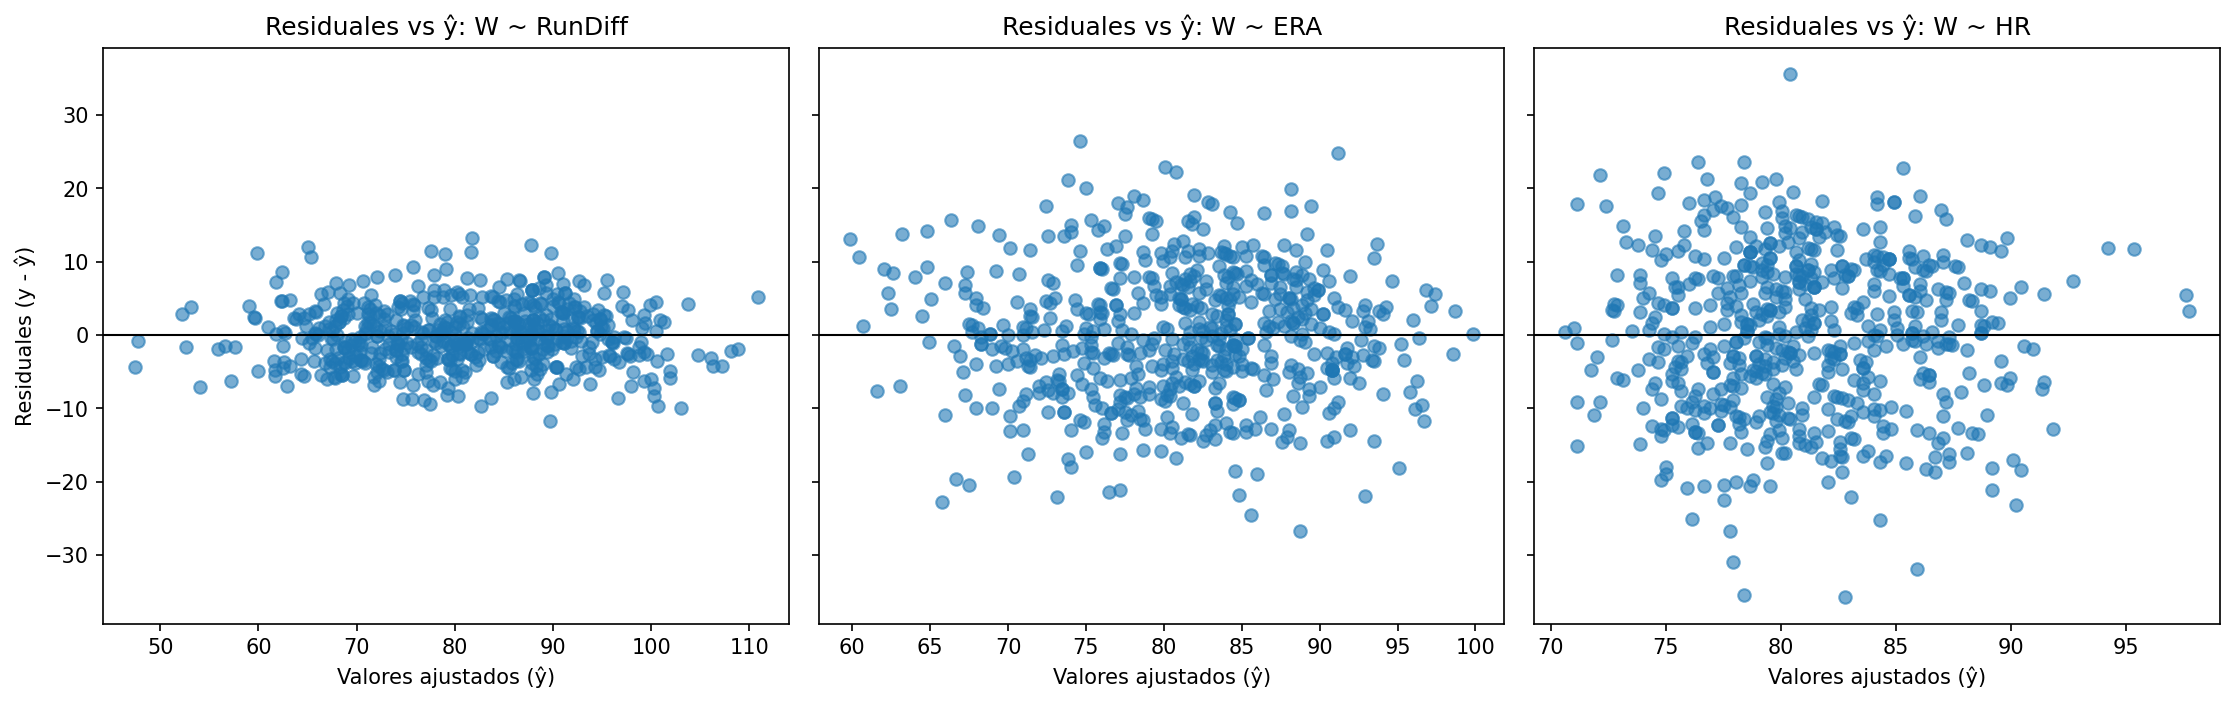
\includegraphics[width=\textwidth]{../plots/ols_resid_grid_RunDiff_ERA_HR.png}
    \caption{Residuales del modelo múltiple vs valores ajustados por predictor.}
\end{figure}

\subsection{Resultados y significancia de coeficientes}
\begin{table}[H]
    \centering
    \caption{Modelo múltiple: $W \sim$ RunDiff + ERA + HR (coeficientes, $p$ e IC95\%)}
    \label{tab:ols_multi_coefs}
    \begin{tabular}{lrrrr}
        \toprule
        \textbf{Variable} & \textbf{$\hat\beta$} & \textbf{$p$-valor} & \textbf{IC95\% inf} & \textbf{IC95\% sup} \\
        \midrule
        Constante & 86.015950 & 0.000000 & 82.550769 & 89.481130 \\
        RunDiff   & 0.091675  & 0.000000 & 0.086527  & 0.096823  \\
        ERA       & -1.824850 & 0.000288 & -2.807436 & -0.842265 \\
        HR        & 0.015600  & 0.008514 & 0.003994  & 0.027206  \\
        \bottomrule
    \end{tabular}
\end{table}

\noindent \textbf{Interpretación de signos y magnitudes.} Manteniendo constantes las demás variables: (i) un incremento de 10 unidades en \texttt{RunDiff} se asocia con \(\approx 0.92\) victorias adicionales; (ii) reducir la \texttt{ERA} en 1.00 se asocia con \(\approx 1.82\) victorias más; (iii) sumar 10 jonrones (\texttt{HR}) se asocia con \(\approx 0.156\) victorias adicionales. Los tres coeficientes son estadísticamente significativos.

\subsection{Bondad de ajuste y pruebas globales}
\begin{table}[H]
    \centering
    \caption{Estadísticos de ajuste y desempeño del modelo múltiple}
    \label{tab:ols_multi_fit}
    \begin{tabular}{lrr}
        \toprule
        Medida & Valor & $p$-valor \\
        \midrule
        $R^2$ & 0.885314 & \\
        $R^2$ ajustado & 0.884737 & \\
        Estadístico $F$ & 1533.603 & 0.000000 \\
        AIC & 3370.731 & \\
        BIC & 3388.319 & \\
        Observaciones ($N$) & 600 & \\
        RMSE & 3.988 & \\
        MAE & 3.177 & \\
        Durbin--Watson & 1.789 & \\
        Omnibus (normalidad) & 4.013 & 0.134 \\
        Jarque--Bera & 3.840 & 0.147 \\
        \bottomrule
    \end{tabular}
\end{table}

\noindent El modelo explica \textbf{88.5\%} de la variación en $W$ (\,$R^2=0.885$\,) con \,$R^2_{adj}=0.885$. La prueba $F(3,596)=1533.60$ es altamente significativa (\,$p<10^{-270}$\,), confirmando relevancia conjunta. Los errores medios de pronóstico in--sample son bajos (RMSE $\approx 3.99$, MAE $\approx 3.18$). Los diagnósticos básicos no rechazan normalidad de residuos (Omnibus/JB, $p>0.10$) y el estadístico Durbin--Watson $\approx 1.79$ no sugiere autocorrelación preocupante en este contexto. El número de condición reportado (\,$\approx 1.98\times10^3$\,) advierte posible \emph{multicolinealidad moderada}; por lo que se complementará con VIF en la sección de supuestos.

\subsection{Comentarios sobre los resultados}
\begin{itemize}
    \item \textbf{RunDiff} es el predictor dominante en magnitud y precisión, consistente con la teoría sabermétrica: resume balance ofensivo--defensivo.
    \item \textbf{ERA} conserva un efecto negativo y significativo una vez controlado RunDiff y HR: mejor pitcheo, más victorias.
    \item \textbf{HR} aporta señal positiva pero de menor tamaño relativo; su significancia indica que, manteniendo constante RunDiff y ERA, el poder de bateo agrega información marginal.
\end{itemize}
%%%%%%%%%%%%%%%%%%%%%%%%%%%%%%%%%%%%%%%%%%%%%%%%%%%%%%%%%%%%%%%%%%%%%%%%%%%%%%%%%%%%%%%%%%%%%%%%%%%%%%%%%%%%%%%%%%%%%%%%%%%%%%%%%%%%%%%%%%%%%%%%%%%%%%%%%%%%%%%%%%%%%%%%%%%%%%%%%%%%%%%%%%%%%%
\section{Validación de los Supuestos de la Regresión Múltiple}
%
\subsection{Linealidad}
La linealidad del modelo se evaluó con gráficos exploratorios y de regresión parcial (Fig.~\ref{fig:partreg}), así como con pruebas formales. El test \textbf{Rainbow} no rechaza la especificación lineal (\emph{p}=0.334). El \textbf{RESET de Ramsey} arroja \emph{p}=0.053, valor cercano al umbral del 5\%; lo consideramos una señal de cautela, pero no evidencia concluyente para modificar la forma funcional. En conjunto, la especificación lineal resulta adecuada para los fines del estudio.

\subsection{Independencia de los errores}
La independencia se contrastó con el estadístico \textbf{Durbin--Watson}, que resultó en \(DW\approx1.79\). Este valor es cercano a 2 y no sugiere autocorrelación de primer orden preocupante en los residuos.

\subsection{Homocedasticidad}
Se revisaron los \emph{residuales vs. valores ajustados} (Fig.~\ref{fig:resid_fitted}) sin patrones de abanico. Las pruebas \textbf{Breusch--Pagan} (\emph{p}=0.26) y \textbf{White} (\emph{p}=0.38) no rechazan la hipótesis nula de varianza constante. Concluimos que no hay evidencia estadística de heterocedasticidad.

\subsection{Normalidad de los residuos}
La normalidad se verificó mediante \textbf{Shapiro--Wilk} (\emph{p}=0.20) y \textbf{Jarque--Bera} (\emph{p}=0.15), que no rechazan normalidad al 5\%. El \emph{QQ-plot} (Fig.~\ref{fig:qqplot}) muestra alineación razonable con la diagonal, con desvíos menores en colas.

\subsection{Ausencia de multicolinealidad}
Se calcularon los \textbf{VIF}: \texttt{RunDiff}\,$\approx$\,3.17, \texttt{ERA}\,$\approx$\,2.68 y \texttt{HR}\,$\approx$\,1.78, todos por debajo de 5, por lo que no hay multicolinealidad grave. El \textbf{número de condición} del diseño es \(\kappa\approx1{,}980\), lo que sugiere colinealidad \emph{moderada}. Esto es esperable porque las métricas de rendimiento de un equipo están naturalmente relacionadas entre sí.

\begin{figure}[H]
    \centering
    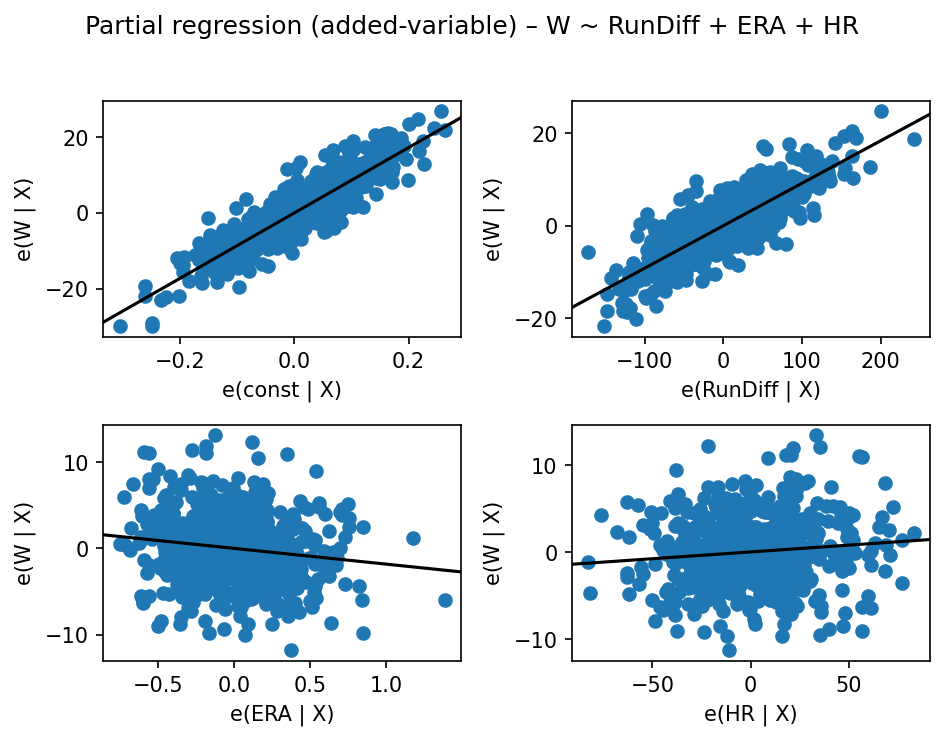
\includegraphics[width=.85\linewidth]{../plots/final_version/ols_partial_regression_grid.png}
    \caption{Regresión parcial (added--variable): grilla de gráficos.}
    \label{fig:partreg}
\end{figure}

\begin{figure}[H]
    \centering
    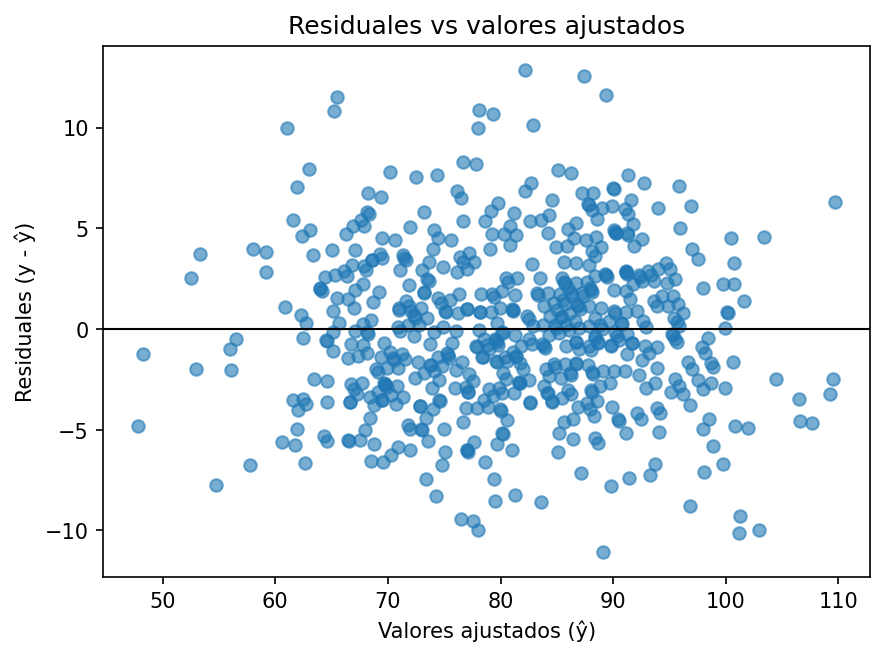
\includegraphics[width=.65\linewidth]{../plots/final_version/ols_residuals_vs_fitted.png}
    \caption{Residuos vs. valores ajustados del modelo múltiple.}
    \label{fig:resid_fitted}
\end{figure}

\begin{figure}[H]
    \centering
    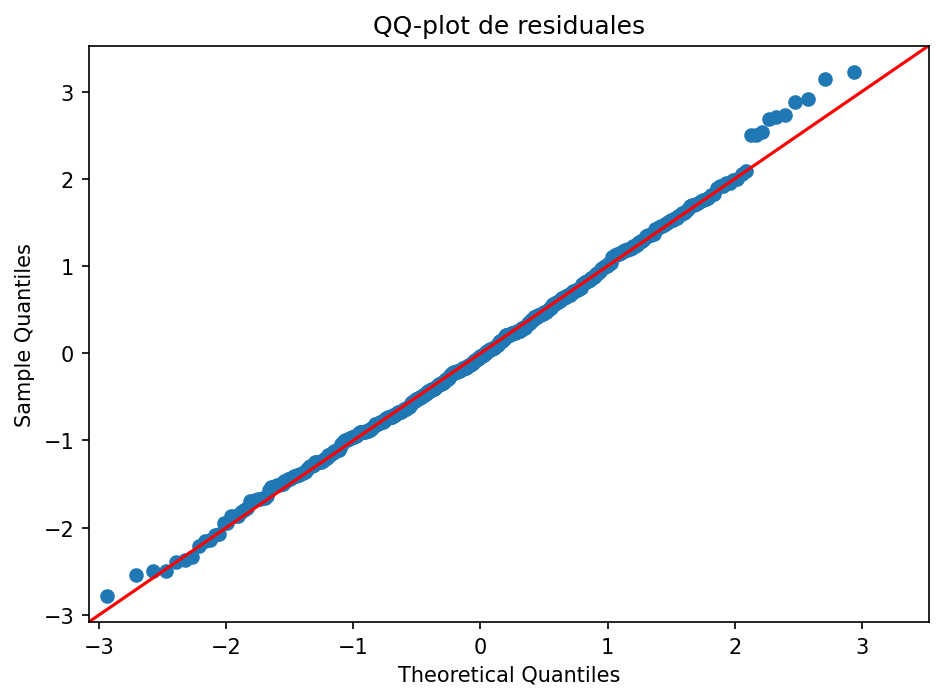
\includegraphics[width=.55\linewidth]{../plots/final_version/ols_residuals_qq.png}
    \caption{QQ-plot de los residuos del modelo.}
    \label{fig:qqplot}
\end{figure}
%%%%%%%%%%%%%%%%%%%%%%%%%%%%%%%%%%%%%%%%%%%%%%%%%%%%%%%%%%%%%%%%%%%%%%%%%%%%%%%%%%%%%%%%%%%%%%%%%%%%%%%%%%%%%%%%%%%%%%%%%%%%%%%%%%%%%%%%%%%%%%%%%%%%%%%%%%%%%%%%%%%%%%%%%%%%%%%%%%%%%%%%%%%%%%
\section{Pronóstico}
\subsection{Generación del pronóstico}
Dividimos el panel equipo–año en un \textit{split} temporal: \emph{entrenamiento} 2000--2016 (510 obs.) y \emph{prueba} 2017--2019 (90 obs.). Con base en la evidencia de ajuste y validación, el modelo usado para pronosticar fue el de mejor desempeño:
\[
\text{W} \;=\; \beta_0 \;+\; \beta_1\,\text{RunDiff} \;+\; \beta_2\,\text{ERA} \;+\; \beta_3\,\text{HR},
\]
ajustado únicamente con el conjunto de entrenamiento y evaluado luego en prueba.

La Figura~\ref{fig:parity_test_best} muestra el \textit{parity plot} (observado vs. pronosticado) en prueba: los puntos se alinean alrededor de la diagonal, lo que refleja buen desempeño predictivo sin sesgos sistemáticos.

\begin{figure}[H]
    \centering
    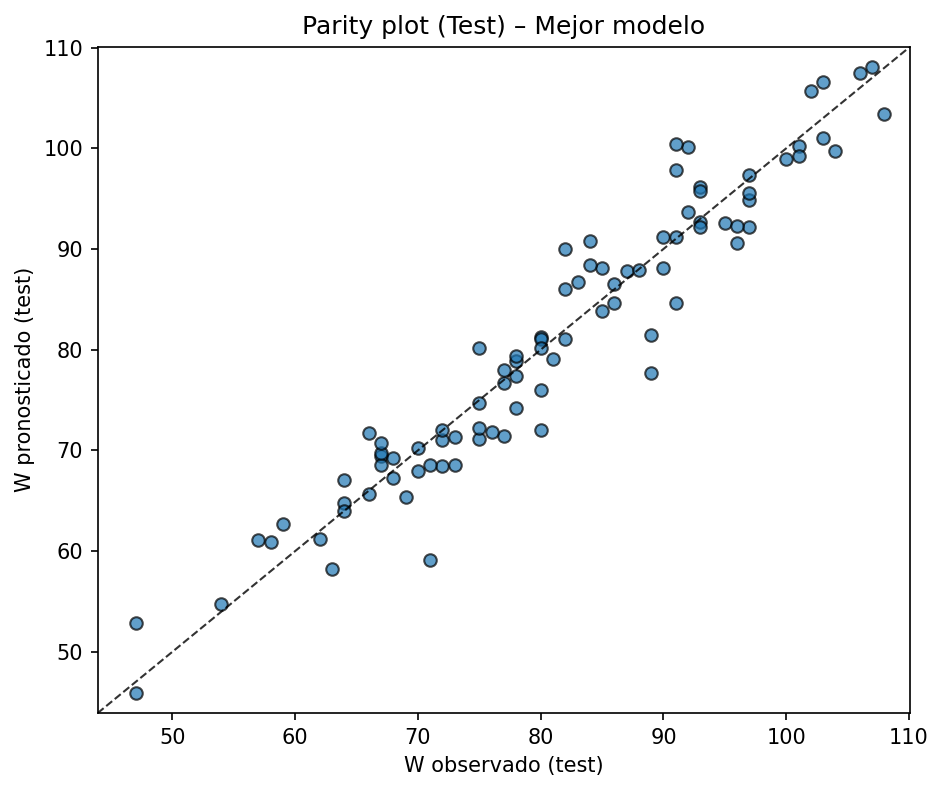
\includegraphics[width=0.6\linewidth]{../plots/forecast_parity_test_best.png}
    \caption{Parity plot (set de prueba) del mejor modelo: $ \text{W} \sim \text{RunDiff} + \text{ERA} + \text{HR} $.}
    \label{fig:parity_test_best}
\end{figure}

\subsection{Intervalos de predicción}
Además del pronóstico puntual $\hat{W}$, reportamos (i) el intervalo de confianza al 95\% para la media condicional y (ii) el intervalo de \emph{predicción} al 95\% para observaciones futuras.

\begin{table}[H]
    \centering
    \caption{Pronósticos puntuales e intervalos (IC 95\% de la media; predicción 95\%).}
    \label{tab:pred_intervals_multi}
    \begin{tabular}{rrrrrrrr}
        \toprule
        RunDiff & ERA & HR & $\hat{W}$ & IC\;95\% inf & IC\;95\% sup & Pred.\;95\% inf & Pred.\;95\% sup \\
        \midrule
        -150 & 5.0 & 140 & 65.11 & 64.39 & 65.83 & 57.19 & 73.03 \\
         -50 & 4.3 & 170 & 76.26 & 75.83 & 76.70 & 68.37 & 84.16 \\
           0 & 4.0 & 200 & 82.02 & 81.31 & 82.74 & 74.11 & 89.94 \\
          50 & 3.8 & 210 & 87.21 & 86.41 & 88.02 & 79.29 & 95.14 \\
         150 & 3.5 & 230 & 97.40 & 96.41 & 98.39 & 89.45 & 105.34 \\
         250 & 3.2 & 250 & 107.58 & 106.33 & 108.82 & 99.60 & 115.56 \\
        \bottomrule
    \end{tabular}
\end{table}
\subsection{Evaluación del pronóstico}
La Tabla~\ref{tab:forecast_metrics} compara el desempeño en entrenamiento y prueba entre el mejor modelo múltiple y tres modelos lineales simples.

\begin{table}[H]
    \centering
    \caption{Desempeño predictivo (MSE, RMSE, MAE) por modelo y partición.}
    \label{tab:forecast_metrics}
    \begin{tabular}{l l r r r r}
        \toprule
        Modelo & Split & MSE & RMSE & MAE & N \\
        \midrule
        Best: W $\sim$ RunDiff + ERA + HR & Train (2000--2016) & 15.98 & 3.998 & 3.205 & 510 \\
        Best: W $\sim$ RunDiff + ERA + HR & Test (2017--2019)  & 15.72 & 3.965 & 3.027 &  90 \\
        RunDiff (lineal)                   & Train (2000--2016) & 16.42 & 4.052 & 3.252 & 510 \\
        RunDiff (lineal)                   & Test (2017--2019)  & 15.57 & 3.946 & 2.978 &  90 \\
        ERA (lineal)                       & Train (2000--2016) & 78.79 & 8.877 & 7.177 & 510 \\
        ERA (lineal)                       & Test (2017--2019)  & 83.49 & 9.137 & 7.209 &  90 \\
        HR (lineal)                        & Train (2000--2016) &109.49 &10.464 & 8.630 & 510 \\
        HR (lineal)                        & Test (2017--2019)  &165.82 &12.877 &10.450 &  90 \\
        \bottomrule
    \end{tabular}
\end{table}

En prueba, el modelo múltiple alcanza RMSE $\approx 3.97$ y MAE $\approx 3.03$, superando claramente a los modelos que usan \emph{una sola} variable y quedando a la par del lineal en RunDiff. Dado que el múltiple integra simultáneamente información de bateo (HR), diferencial agregado (RunDiff) y pitcheo (ERA), ofrece una \emph{mejor base explicativa} con errores similares o menores.

Finalmente, verificamos los residuales del modelo en el set de prueba (Fig.~\ref{fig:resid_fitted_test}): la nube se distribuye alrededor de cero sin patrón de abanico, lo cual es consistente con la homocedasticidad indicada por las pruebas.

\begin{figure}[H]
    \centering
    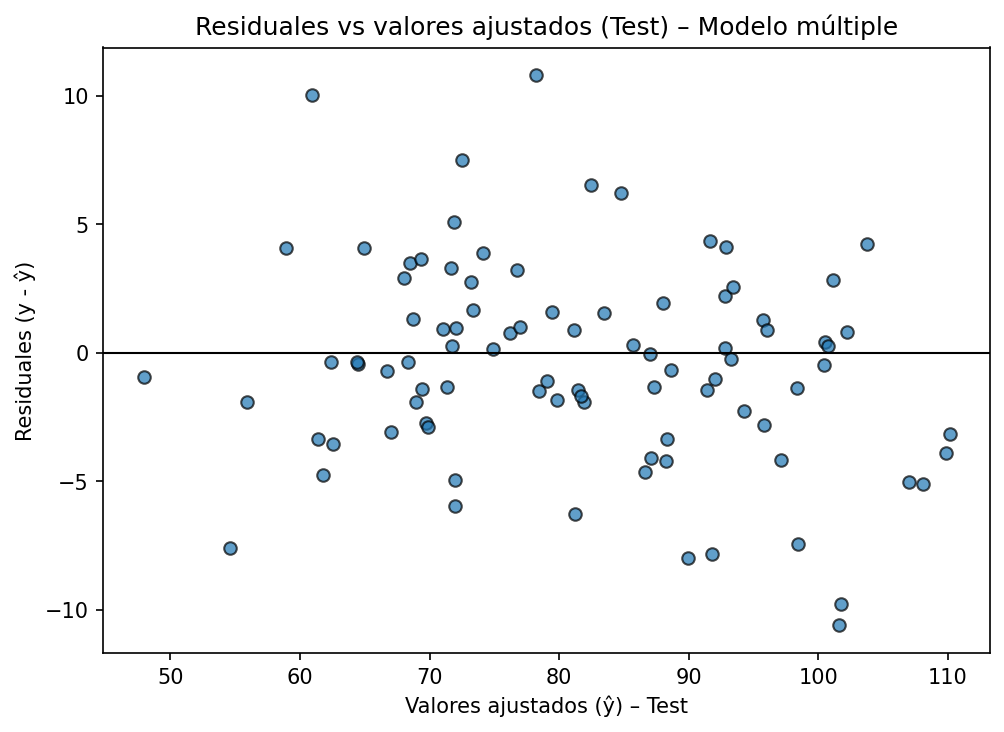
\includegraphics[width=0.8\linewidth]{../plots/final_version/forecast_residuals_vs_fitted_test.png}
    \caption{Residuos vs. valores ajustados (Test) – Modelo múltiple.}
    \label{fig:resid_fitted_test}
\end{figure}
%%%%%%%%%%%%%%%%%%%%%%%%%%%%%%%%%%%%%%%%%%%%%%%%%%%%%%%%%%%%%%%%%%%%%%%%%%%%%%%%%%%%%%%%%%%%%%%%%%%%%%%%%%%%%%%%%%%%%%%%%%%%%%%%%%%%%%%%%%%%%%%%%%%%%%%%%%%%%%%%%%%%%%%%%%%%%%%%%%%%%%%%%%%%%%
\section{Conclusiones}
\subsection{Resumen de resultados}
El modelo de \textbf{regresión lineal múltiple} \(W \sim \text{RunDiff} + \text{ERA} + \text{HR}\) explica el \textbf{88.5\%} de la variación en las victorias por temporada (\(R^2=0.885\); \(R^2_{aj}=0.885\)). La prueba global \(F(3,596)=1533.60\; (p<10^{-270})\) confirma la \emph{relevancia conjunta} de los predictores.

En términos de \emph{efectos parciales} (manteniendo constantes las demás variables):
\begin{itemize}
    \item \textbf{RunDiff}: coeficiente \(\hat\beta\approx0.0917\). Un aumento de 10 carreras en el diferencial se asocia con \(\approx0.92\) victorias adicionales. Es el predictor con mayor precisión y magnitud relativa.
    \item \textbf{ERA}: coeficiente \(\hat\beta\approx-1.825\). Reducir la efectividad en 1.00 se asocia con \(\approx1.82\) victorias más, consistente con el papel del pitcheo en el desempeño global.
    \item \textbf{HR}: coeficiente \(\hat\beta\approx0.0156\). Sumar 10 jonrones se asocia con \(\approx0.156\) victorias adicionales; el efecto es positivo pero de menor tamaño que \texttt{RunDiff} y \texttt{ERA}.
\end{itemize}

Los diagnósticos apoyan la validez del modelo para los fines del estudio: \textbf{DW}\(\approx1.79\) no sugiere autocorrelación de primer orden; \textbf{Omnibus/JB} no rechazan normalidad (\(p>0.10\)); \textbf{BP} y \textbf{White} no rechazan homocedasticidad (\(p=0.26\) y \(p=0.38\)). Los \textbf{VIF} (\(\approx3.17, 2.68, 1.78\)) y el número de condición (\(\kappa\approx1{,}980\)) indican colinealidad \emph{moderada}, esperable en métricas de rendimiento de un mismo equipo.

En evaluación temporal, el modelo múltiple alcanzó en prueba (2017--2019) \(\text{RMSE}\approx3.97\) y \(\text{MAE}\approx3.03\), con buen alineamiento observado–pronosticado y residuales sin patrones sistémicos, lo que respalda su uso para pronóstico de corto plazo.

\subsection{Recomendaciones}
\begin{enumerate}
    \item \textbf{Uso práctico del modelo.} Emplear \(W \sim \text{RunDiff} + \text{ERA} + \text{HR}\) para pronósticos explicables y consistentes. Reportar siempre el error típico (RMSE/MAE) como referencia operativa.
    \item \textbf{Comunicación de incertidumbre.} Acompañar cada pronóstico puntual \(\hat W\) con su \textbf{intervalo de predicción al 95\%}; evitar interpretar el IC de la media como incertidumbre individual.
    \item \textbf{Monitoreo de supuestos.} Mantener verificación periódica de linealidad, homocedasticidad y normalidad; ante señales de heteroscedasticidad, complementar con errores estándar robustos (HC3) como sensibilidad.
    \item \textbf{Colinealidad.} Vigilar VIF y el número de condición al incorporar nuevas variables; priorizar parsimonia para preservar estabilidad de coeficientes e interpretabilidad.
    \item \textbf{Mantenimiento del modelo.} Reentrenar con datos recientes (p. ej., anual) y validar con \emph{split} temporal; considerar \emph{rolling-origin} cuando el objetivo principal sea pronóstico.
    \item \textbf{Extensiones posibles.} Explorar especificaciones de panel con efectos fijos por franquicia/año y la inclusión de métricas complementarias (BB, SO, OBP, SLG) para descomponer aportes ofensivos y de pitcheo, evaluando siempre el impacto en VIF y desempeño predictivo.
\end{enumerate}
%%%%%%%%%%%%%%%%%%%%%%%%%%%%%%%%%%%%%%%%%%%%%%%%%%%%%%%%%%%%%%%%%%%%%%%%%%%%%%%%%%%%%%%%%%%%%%%%%%%%%%%%%%%%%%%%%%%%%%%%%%%%%%%%%%%%%%%%%%%%%%%%%%%%%%%%%%%%%%%%%%%%%%%%%%%%%%%%%%%%%%%%%%%%%%
\section{Bibliografía}
Lahman Baseball Database -Society for American Baseball Research. (2025). Sabr.org. \url{https://sabr.org/lahman-database/}
%%%%%%%%%%%%%%%%%%%%%%%%%%%%%%%%%%%%%%%%%%%%%%%%%%%%%%%%%%%%%%%%%%%%%%%%%%%%%%%%%%%%%%%%%%%%%%%%%%%%%%%%%%%%%%%%%%%%%%%%%%%%%%%%%%%%%%%%%%%%%%%%%%%%%%%%%%%%%%%%%%%%%%%%%%%%%%%%%%%%%%%%%%%%%%
%%%%%%%%%%%%%%%%%%%%%%%%%%%%%%%%%%%%%%%%%%%%%%%%%%%%%%%%%%%%%%%%%%%%%%%%%%%%%%%%%%%%%%%%%%%%%%%%%%%%%%%%%%%%%%%%%%%%%%%%%%%%%%%%%%%%%%%%%%%%%%%%%%%%%%%%%%%%%%%%%%%%%%%%%%%%%%%%%%%%%%%%%%%%%%
\section{Anexo}
\subsection{Link al repositorio con código fuente y salidas correspondientes}
\url{https://github.com/enriquegomeztagle/MCD-ProyectoFinalEconometria-DeterminantesVictoriasMLB}
%%%%%%%%%%%%%%%%%%%%%%%%%%%%%%%%%%%%%%%%%%%%%%%%%%%%%%%%%%%%%%%%%%%%%%%%%%%%%%%%%%%%%%%%%%%%%%%%%%%%%%%%%%%%%%%%%%%%%%%%%%%%%%%%%%%%%%%%%%%%%%%%%%%%%%%%%%%%%%%%%%%%%%%%%%%%%%%%%%%%%%%%%%%%%%
%%%%%%%%%%%%%%%%%%%%%%%%%%%%%%%%%%%%%%%%%%%%%%%%%%%%%%%%%%%%%%%%%%%%%%%%%%%%%%%%%%%%%%%%%%%%%%%%%%%%%%%%%%%%%%%%%%%%%%%%%%%%%%%%%%%%%%%%%%%%%%%%%%%%%%%%%%%%%%%%%%%%%%%%%%%%%%%%%%%%%%%%%%%%%%
\end{document}
%%%%%%%%%%%%%%%%%%%%%%%%%%%%%%%%%%%%%%%%%%%%%%%%%%%%%%%%%%%%%%%%%%%%%%%%%%%%%%%%%%%%%%%%%%%%%%%%%%%%%%%%%%%%%%%%%%%%%%%%%%%%%%%%%%%%%%%%%%%%%%%%%%%%%%%%%%%%%%%%%%%%%%%%%%%%%%%%%%%%%%%%%%%%%%
